\documentclass{tufte-handout}

%\geometry{showframe}% for debugging purposes -- displays the margins

\usepackage{amsmath}

% Set up the images/graphics package
\usepackage{graphicx}
\setkeys{Gin}{width=\linewidth,totalheight=\textheight,keepaspectratio}
\graphicspath{{graphics/}}


% The following package makes prettier tables.  We're all about the bling!
\usepackage{booktabs}

% The units package provides nice, non-stacked fractions and better spacing
% for units.
\usepackage{units}

% The fancyvrb package lets us customize the formatting of verbatim
% environments.  We use a slightly smaller font.
\usepackage{fancyvrb}
\fvset{fontsize=\normalsize}

% Small sections of multiple columns
\usepackage{multicol}

% Provides paragraphs of dummy text
\usepackage{lipsum}

% Provides annotated music scores
\usepackage{musicography}

% Fancy header
\usepackage{fancyhdr}

\usepackage{array, boldline, makecell, booktabs}

\newcommand{\bmp}[1]{\begin{minipage}{#1}}
\newcommand{\emp}{\end{minipage}}
\newcommand{\tw}{\textwidth}

% These commands are used to pretty-print LaTeX commands
\newcommand{\doccmd}[1]{\texttt{\textbackslash#1}}% command name -- adds backslash automatically
\newcommand{\docopt}[1]{\ensuremath{\langle}\textrm{\textit{#1}}\ensuremath{\rangle}}% optional command argument
\newcommand{\docarg}[1]{\textrm{\textit{#1}}}% (required) command argument
\newenvironment{docspec}{\begin{quote}\noindent}{\end{quote}}% command specification environment
\newcommand{\docenv}[1]{\textsf{#1}}% environment name
\newcommand{\docpkg}[1]{\texttt{#1}}% package name
\newcommand{\doccls}[1]{\texttt{#1}}% document class name
\newcommand{\docclsopt}[1]{\texttt{#1}}% document class option name


%%% Additions to template by DSL
\usepackage{hyperref} % provides \url{}
% remove separation between list items http://tex.stackexchange.com/a/10689/1783
\usepackage{enumitem}
\setlist{nosep}

%%-- another way
\usepackage{tikzpagenodes}
\newcommand{\mylogo}[1]{%
\tikz[remember picture,overlay] {%
  \node[inner sep=0pt,anchor=east] at ([yshift=+1.0cm, xshift=+7.0cm]current page text area.north east){#1};}
  }

\usepackage{mathrsfs}
\usepackage{tcolorbox}
\tcbuselibrary{theorems}
\usepackage{xcolor}
\usepackage{epsdice}
\usepackage{pgfplots}

\usepackage{graphicx,xspace,color,cancel}
\usepackage{tikz}
\usetikzlibrary{arrows,shapes,backgrounds,through,shadows}
\usetikzlibrary{decorations.pathmorphing}
\usetikzlibrary{calc}

\newcommand{\boxit}[4]
{
\path #2+(-#4,-#4) node(bottomleft){};
\path #3+(#4,#4) node(upperright){};
\draw[rounded corners,black!80] (bottomleft) rectangle (upperright);
%\path (#2-|#3) node(bottomright){};
\path (bottomleft-|upperright) node(bottomright){};
\path (bottomright) node[above left]{#1};
}

\tikzstyle{cont}=[circle, draw,% a shading that is white at the top...
thick,minimum size=6mm,line width=1pt,>=stealth]  % continuous  node
\tikzstyle{dgraph}=[->, line width=1.5pt]
\tikzstyle{ugraph}=[line width=1.5pt]

\tikzstyle{contblk}=[circle, draw=black,top color=black,bottom color=black,% a shading that is white at the top...
thick,minimum size=1mm,line width=1pt,>=stealth]  % continuous  node
\tikzstyle{dgraph}=[->, line width=1.5pt]



\newtcbtheorem[number within=]{mydef}{Definition}%
{colback=DarkOrchid!5,colframe=DarkOrchid!90!black,fonttitle=\bfseries}{th}

\newtcbtheorem[number within=]{mydef2}{Definition$^*$}%
{colback=Rhodamine!5,colframe=Rhodamine!90!black,fonttitle=\bfseries}{th}


\newtcbtheorem[number within=]{mybox}{Box}%
{colback=Aquamarine!5,colframe=Aquamarine!90!black,fonttitle=\bfseries}{th}

\newtcbtheorem[number within=]{mybox2}{Box$^*$}%
{colback=gray!5,colframe=gray!90!black,fonttitle=\bfseries}{th}

\newtcbtheorem[number within=]{mythe}{Theorem}%
{colback=DarkOrchid!5,colframe=DarkOrchid!90!black,fonttitle=\bfseries}{th}






% \bigcupdot
\makeatletter
\def\moverlay{\mathpalette\mov@rlay}
\def\mov@rlay#1#2{\leavevmode\vtop{%
   \baselineskip\z@skip \lineskiplimit-\maxdimen
   \ialign{\hfil$\m@th#1##$\hfil\cr#2\crcr}}}
\newcommand{\charfusion}[3][\mathord]{
    #1{\ifx#1\mathop\vphantom{#2}\fi
        \mathpalette\mov@rlay{#2\cr#3}
      }
    \ifx#1\mathop\expandafter\displaylimits\fi}
\makeatother
\newcommand{\cupdot}{\charfusion[\mathbin]{\cup}{\cdot}}
\newcommand{\bigcupdot}{\charfusion[\mathop]{\bigcup}{\boldsymbol{\cdot}}}


\usepackage{amsmath}
\usepackage{amssymb}
\usepackage{algorithm}
\usepackage{algpseudocode}
\usepackage{geometry}
\usepackage{hyperref}
\usepackage{listings}
\usepackage{xcolor}



\lstset{
    language=Python,
    basicstyle=\ttfamily\small,
    keywordstyle=\color{blue},
    commentstyle=\color{green!60!black},
    stringstyle=\color{orange},
    showstringspaces=false,
    breaklines=true,
    frame=single,
    numbers=left,
    numberstyle=\tiny\color{gray}
}


%\rhead{\includegraphics[width=1cm]{fig/T1.png}}
\def\ci{\perp\!\!\!\perp}

\title{Multilayer Perceptron }
\author{Salvador Ruiz Correa}
\date{Nov 29, 2024}  % if the \date{} command is left out, the current date will be used
\begin{document}

\maketitle% this prints the handout title, author, and date
\mylogo{
\includegraphics[height=15mm]{fig/T2.png}}

\begin{abstract}
\noindent \textsc{A multilayer perceptron} (MLP) is a type of artificial neural network (ANN) consisting of multiple layers of nodes, with each layer fully connected to the next layer. It typically comprises an input layer, one or more hidden layers, and an output layer. Each node in the hidden layers and the output layer applies a nonlinear activation function to the weighted sum of its inputs, allowing the network to learn complex relationships in the data. MLPs are commonly used for supervised learning tasks such as classification and regression. They are trained using techniques like backpropagation, adjusting the weights of connections between nodes to minimize the difference between the predicted output and the actual output.\end{abstract}
\marginnote[-5cm]{
\textsc{Agenda:}
\begin{description}
\item{1} Multilayer Perceptron.
\item{2} Backpropagation.
\item{3} Gradient Descent.
\item{4} Curse of Dimensionality.
\item{5} Separation Theorem.
\item{5} Kernel Trick


\end{description}
}



\section{Regression Model}

We start by discussing regression problems. We begin by considering a generative model where
the target forma a multivariate Gaussian vector  $\mathcal N(\mathbf t\mid \boldsymbol \mu(\mathbf x), \beta^{-1}\mathbf I)$,
where $\mathbf I$ is a diagonal matrix and  $\beta $ is the precision (inverse of the variance). We are given a set of input vectors $\{\mathbf X_1, \mathbf X_2, \dots, \mathbf X_N\}$ and the corresponding target vectors $\{\mathbf T_1, \mathbf T_2, \dots, \mathbf T_N\}$. See Figure \ref{fig:sin} for a simple example.

\begin{marginfigure}
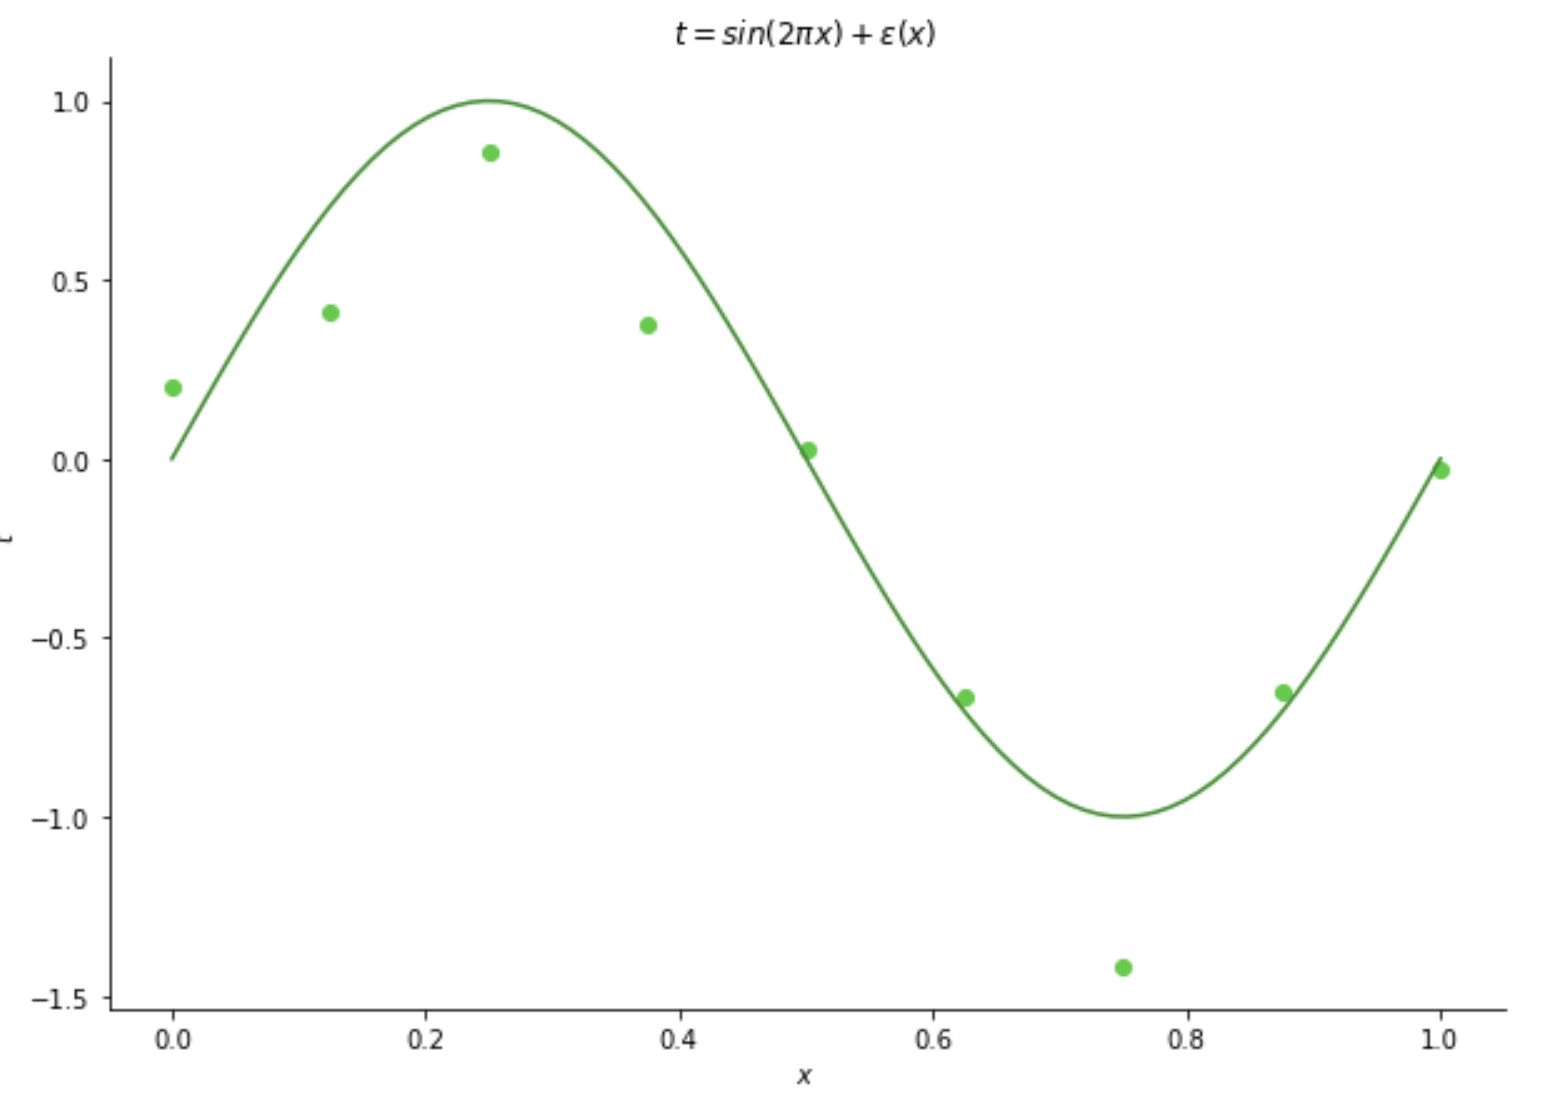
\includegraphics{fig/signal.png}
\label{fig:sin}
\caption{Green dots represent data samples computed as $t=\sin(2\pi x) + \epsilon(x)$, for a set of $x$ input data where $\epsilon$ represents a normal {\em random noise} of mean zero and variance $\sigma^2$.   Notice that the probability density of the target variable is $\mathcal N(t\mid \sin(2\pi x), \sigma^2)$.  }
\end{marginfigure}


To solve the regression model, we approximate the mean vector $\mu(\mathbf x)$ with the random vectors $\mathbf Y$   as depicted given by the following probability density for the target variables is  $\mathcal N(\mathbf t\mid \boldsymbol y(\mathbf x, \mathbf w), \beta^{-1}\mathbf I)$. 

\begin{center}
\scalebox{0.8}{
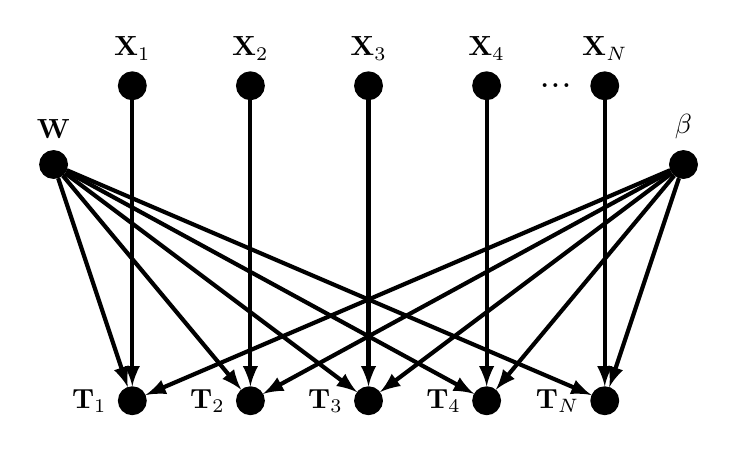
\begin{tikzpicture}[dgraph]
\node[contblk,label=above:{$\mathbf W$}] (W) at (-1.,0) {};
\node[contblk,label=above:{$\beta$}] (B) at (7,0) {};
\node[contblk,label=above:{$\mathbf X_1$}] (x1) at (0,1) {};
\node[contblk, label=above:{$\mathbf X_2$}] (x2) at (1.5, 1) {};
\node[contblk, label=above:{$\mathbf X_3$}] (x3) at (3,1) {};
\node[contblk, label=above:{$\mathbf X_4$}] (x4) at (4.5,1) {};
\node[contblk, label=above:{$\mathbf X_N$}] (xN) at (6,1) {};
%\node[contblk,label=left:{$\mathbf Y_1$}] (y1) at (0,-2) {};
%\node[contblk, label=left:{$\mathbf Y_2$}] (y2) at (1.5, -2) {};
%\node[contblk, label=left:{$\mathbf Y_3$}] (y3) at (3,-2) {};
%\node[contblk, label=left:{$\mathbf Y_4$}] (y4) at (4.5,-2) {};
%\node[contblk, label=left:{$\mathbf Y_N$}] (yN) at (6,-2) {};
\node[contblk,label=left:{$\mathbf T_1$}] (t1) at (0,-3) {};
\node[contblk, label=left:{$\mathbf T_2$}] (t2) at (1.5, -3) {};
\node[contblk, label=left:{$\mathbf T_3$}] (t3) at (3,-3) {};
\node[contblk, label=left:{$\mathbf T_4$}] (t4) at (4.5,-3) {};
\node[contblk, label=left:{$\mathbf T_N$}] (tN) at (6,-3) {};
\path (x4) -- (xN) node [black, font=\Large, midway] {$\,\,\,...$};
\draw [-{latex[slant=0]}]  (W) -- (t1);
\draw [-{latex[slant=0]}]  (W) -- (t2);
\draw [-{latex[slant=0]}]  (W) -- (t3);
\draw [-{latex[slant=0]}]  (W) -- (t4);
\draw [-{latex[slant=0]}]  (W) -- (tN);
\draw [-{latex[slant=0]}]  (B) -- (t1);
\draw [-{latex[slant=0]}]  (B) -- (t2);
\draw [-{latex[slant=0]}]  (B) -- (t3);
\draw [-{latex[slant=0]}]  (B) -- (t4);
\draw [-{latex[slant=0]}]  (B) -- (tN);
\draw [-{latex[slant=0]}]  (x1) -- (t1);
\draw [-{latex[slant=0]}]  (x2) -- (t2);
\draw [-{latex[slant=0]}]  (x3) -- (t3);
\draw [-{latex[slant=0]}]  (x4) -- (t4);
\draw [-{latex[slant=0]}]  (xN) -- (tN);
%\draw [-{latex[slant=0]}]  (y1) -- (t1);
%\draw [-{latex[slant=0]}]  (y2) -- (t2);
%\draw [-{latex[slant=0]}]  (y3) -- (t3);
%\draw [-{latex[slant=0]}]  (y4) -- (t4);
%\draw [-{latex[slant=0]}]  (yN) -- (tN);
\end{tikzpicture}
}
\end{center}

We will use a neural network model that uses a solution space of the form:

\begin{align*}
\mathcal H_{\mathbf w} = \{ y_k(\mathbf x_n, \mathbf w)\,\,, k=1,2,\dots,K\},
\end{align*}
where
\begin{align*}
y_k(\mathbf x, \mathbf w) =  \sum_{j=0}^{M_L} w_{kj}^{L}\,h^L \left(\cdots \sum_{r=0}^{M_2} w_{sr}^{2}\,  h^2\left(\sum_{q=0}^{M_1} w_{rq}^{1}\, h^1\left(  \sum_{i=0}^{M_0} w_{qi}^{0}x_i \right) \right) \right).
\end{align*}
and $h^l$, $l=1,2,\dots,L$, is an activation function.
Notice that the term
\begin{align*}
h^L\left(\cdots \sum_{r=0}^{M_2} w_{sr}^{2}\,  h\left(\sum_{q=0}^{M_1} w_{rq}^{1}\, h\left(  \sum_{i=0}^{M_0} w_{qi}^{0}x_i \right) \right) \right)
\end{align*}
depends on the $j$ index.
Notice that there is a total  of $$\sum_{l=0}^{L+1} M_l \times M_{l-1}$$
random variables $\mathbf W$. 

First, we will use the frequentist approach to solve the regression problem using a neural network by assuming that the vectors $\mathbf w$  and $\beta$ are parameters that need to be estimated using the MLE approach.

\begin{center}
\scalebox{0.8}{
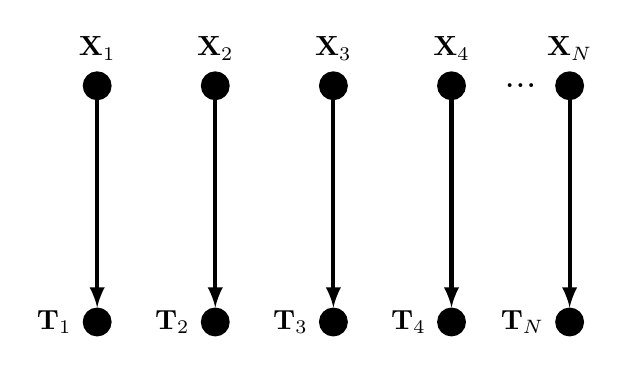
\begin{tikzpicture}[dgraph]


\node[contblk,label=above:{$\mathbf X_1$}] (x1) at (0,1) {};
\node[contblk, label=above:{$\mathbf X_2$}] (x2) at (1.5, 1) {};
\node[contblk, label=above:{$\mathbf X_3$}] (x3) at (3,1) {};
\node[contblk, label=above:{$\mathbf X_4$}] (x4) at (4.5,1) {};
\node[contblk, label=above:{$\mathbf X_N$}] (xN) at (6,1) {};

\node[contblk,label=left:{$\mathbf T_1$}] (t1) at (0,-2) {};
\node[contblk, label=left:{$\mathbf T_2$}] (t2) at (1.5, -2) {};
\node[contblk, label=left:{$\mathbf T_3$}] (t3) at (3,-2) {};
\node[contblk, label=left:{$\mathbf T_4$}] (t4) at (4.5,-2) {};
\node[contblk, label=left:{$\mathbf T_N$}] (tN) at (6,-2) {};
\path (x4) -- (xN) node [black, font=\Large, midway] {$\,\,\,...$};

\draw [-{latex[slant=0]}]  (x1) -- (t1);
\draw [-{latex[slant=0]}]  (x2) -- (t2);
\draw [-{latex[slant=0]}]  (x3) -- (t3);
\draw [-{latex[slant=0]}]  (x4) -- (t4);
\draw [-{latex[slant=0]}]  (xN) -- (tN);

\end{tikzpicture}
}
\end{center}

That is, we have that the target vector $\mathbf t$ is distributed according to  $\mathcal N(\mathbf t; \boldsymbol y(\mathbf x, \mathbf w), \beta^{-1}\mathbf I)$, where $\mathbf w$ and $\beta$ are the probability density parameters.



\vspace{-0\baselineskip}\footnotetext{Source:Bishop. (2006). Pattern Recognition and Machine Learning, Springer.}
\vspace{0\baselineskip}

\section{Multilayer Perceptron}

We introduce the MLP function family using a simple example. Assume that we have an i.i.d. data set
$\mathcal D = \{(\mathbf x_1, \mathbf t_1), (\mathbf x_2, \mathbf t_2), \dots, (\mathbf x_N, \mathbf t_N)\}$
where $\mathbf x_n = (x_{n1}, x_{n2}  )$, and $\mathbf t_n = (t_{n1}, t_{n2} )$.
The probability density of $\mathbf T_n$ given  $\mathbf X_n$ is $p(\mathbf t_n\mid \mathbf  x_n) =\mathcal N(\mathbf t_n; \mathbf y(\mathbf x_n, \mathbf w), \sigma^{2}\mathbf I))$ where $\beta = \sigma^{-2}$ is the precision.

\begin{figure}[t!]
\begin{center}
\scalebox{0.8}{
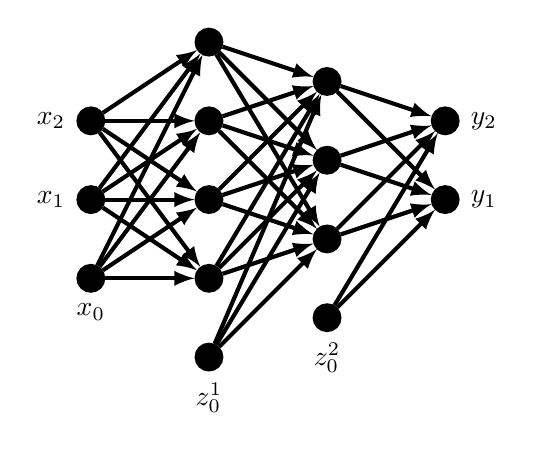
\begin{tikzpicture}[dgraph]

\node[contblk,label=below:{$x_0$}] (x0) at (0,0) {};
\node[contblk, label=left:{$x_1$}] (x1) at (0,1 ) {};
\node[contblk, label=left:{$x_2$}] (x2) at (0,2 ) {};

\node[contblk,label=below:{$z^1_0$}] (z0) at (1.5,-1) {};
\node[contblk,label=left:{}] (z1) at (1.5,0) {};
\node[contblk, label=left:{}] (z2) at (1.5,1 ) {};
\node[contblk, label=left:{}] (z3) at (1.5,2 ) {};
\node[contblk,label=left:{}] (z4) at (1.5,3) {};

\node[contblk,label=left:{}] (zz3) at (3,2.5) {};
\node[contblk,label=left:{}] (zz2) at (3,1.5) {};
\node[contblk,label=left:{}] (zz1) at (3,0.5) {};
\node[contblk,label=below:{$z^2_0$}] (zz0) at (3,-0.5) {};


\node[contblk,label=right:{$y_2$}] (y2) at (4.5,2) {};
\node[contblk,label=right:{$y_1$}] (y1) at (4.5,1) {};

%\draw [-{latex[slant=0]}]  (x0) -- (z0);
%\draw [-{latex[slant=0]}]  (x1) -- (z0);
%\draw [-{latex[slant=0]}]  (x2) -- (z0);
\draw [-{latex[slant=0]}]  (x0) -- (z1);
\draw [-{latex[slant=0]}]  (x1) -- (z1);
\draw [-{latex[slant=0]}]  (x2) -- (z1);
\draw [-{latex[slant=0]}]  (x0) -- (z2);
\draw [-{latex[slant=0]}]  (x1) -- (z2);
\draw [-{latex[slant=0]}]  (x2) -- (z2);
\draw [-{latex[slant=0]}]  (x0) -- (z3);
\draw [-{latex[slant=0]}]  (x1) -- (z3);
\draw [-{latex[slant=0]}]  (x2) -- (z3);
\draw [-{latex[slant=0]}]  (x0) -- (z4);
\draw [-{latex[slant=0]}]  (x1) -- (z4);
\draw [-{latex[slant=0]}]  (x2) -- (z4);

%\draw [-{latex[slant=0]}]  (z0) -- (zz0);
%\draw [-{latex[slant=0]}]  (z1) -- (zz0);
%\draw [-{latex[slant=0]}]  (z2) -- (zz0);
%\draw [-{latex[slant=0]}]  (z3) -- (zz0);
%\draw [-{latex[slant=0]}]  (z4) -- (zz0);
\draw [-{latex[slant=0]}]  (z0) -- (zz1);
\draw [-{latex[slant=0]}]  (z1) -- (zz1);
\draw [-{latex[slant=0]}]  (z2) -- (zz1);
\draw [-{latex[slant=0]}]  (z3) -- (zz1);
\draw [-{latex[slant=0]}]  (z4) -- (zz1);
\draw [-{latex[slant=0]}]  (z0) -- (zz2);
\draw [-{latex[slant=0]}]  (z1) -- (zz2);
\draw [-{latex[slant=0]}]  (z2) -- (zz2);
\draw [-{latex[slant=0]}]  (z3) -- (zz2);
\draw [-{latex[slant=0]}]  (z4) -- (zz2);
\draw [-{latex[slant=0]}]  (z0) -- (zz3);
\draw [-{latex[slant=0]}]  (z1) -- (zz3);
\draw [-{latex[slant=0]}]  (z2) -- (zz3);
\draw [-{latex[slant=0]}]  (z3) -- (zz3);
\draw [-{latex[slant=0]}]  (z4) -- (zz3);

\draw [-{latex[slant=0]}]  (zz0) -- (y1);
\draw [-{latex[slant=0]}]  (zz1) -- (y1);
\draw [-{latex[slant=0]}]  (zz2) -- (y1);
\draw [-{latex[slant=0]}]  (zz3) -- (y1);
\draw [-{latex[slant=0]}]  (zz0) -- (y2);
\draw [-{latex[slant=0]}]  (zz1) -- (y2);
\draw [-{latex[slant=0]}]  (zz2) -- (y2);
\draw [-{latex[slant=0]}]  (zz3) -- (y2);


\end{tikzpicture}
}
\end{center}
\label{fig:nn}
\caption{Multilayer perceptron used to represent the function $\mathbf y(\cdot,\cdot)$.}
\end{figure}


The  likelihood of the data is
\begin{align*}
\prod_{n=1}^N p(\mathbf t_n\mid \mathbf  x_n) &=  \prod_{n=1}^N  (2\pi)^{-1}  \beta \exp \left(-\frac{\beta}{2}  \mid\mid \mathbf t_n -  \mathbf y(\mathbf x_n, \mathbf w) \mid\mid^2 \right).
\end{align*}
The negative of the likelihood is 
\begin{align*}
\mathrm E(\mathbf w,\beta) &= -\log \prod_{n=1}^N p(\mathbf t_n\mid \mathbf  x_n)\\ &=  \frac{\beta}{2}  \sum_{n=1}^N   \mid\mid \mathbf t_n -  \mathbf y(\mathbf x_n, \mathbf w) \mid\mid^2  - N \log \beta  + N \log (2\pi)\\
&=  \frac{\beta}{2}  \sum_{n=1}^N \sum_{i=1}^2 \left( t_{ni} -  y_i(\mathbf x_n, \mathbf w) \right)^2 - N \log \beta  + N \log (2\pi)
\end{align*}

The mean vector of the distribution is represented by the function  $\mathbf y(\cdot,\cdot)$, which corresponds to the computational structure depicted in Figure \ref{fig:nn}.

This neural network has $L=4$ layers $(0,1,2,3)$, including the input, output, and two hidden layers. For the reasons below, we use the auxiliary variables $x_0$, $ z^1_0$, and $ z2_0$.
The  $i$-th node of one layer (i.e., the $i$-th artificial neuron) connects to the $j$ row of the consecutive layer  (say layer $l$) through a weight $$w^l_{ji} = w^l_{i\rightarrow j}.$$ Nodes $x_0$, $z^1_0$, and $z^2_0$ do not receive 
connections from the previous layer, as shown in Figure \ref{fig:nn}.  Notice that each neuron in the hidden and output layers is fully connected to the neurons of the previous layer.

The key idea is to find the network weights that minimize the data's minus log-likelihood. Namely, we want to find 
an  MLE solution to the problem. 

For now, we assume that the precision $\beta$ is given.  Therefore, we want to  minimize:
\begin{align*}
\mathrm E(\mathbf w) &=  \frac{1}{2}\sum_{n=1}^N \sum_{i=1}^2 \left( t_{ni} -  y_i(\mathbf x_n, \mathbf w) \right)^2 \\
&=  \sum_{n=1}^N \mathrm E_n(\mathbf w).
\end{align*}
To find the MLE solution using SGD, we need to understand 
how data is processed in the network and how to compute the gradient of $\mathrm E(\mathbf w)$. In what follows,
we omit the subscript $n$ to avoid cluttering notation.


\subsection{Forward Propagation}
We start by computing the output of each neuron in the hidden and the output layers, often called forward propagation or forward pass. Each output (say the $j$-the neuron in of the $l$ layer) is calculated in two stages.
\begin{itemize}
\item First, incoming data from the previous layer is transformed using an affine transformation.
\begin{align}
a_j^l &= \sum_{\forall i \rightarrow j} w^l_{ji}z^{l-1}_i  \\ 
&= \sum_{i=0 }^{M_l-1} w^l_{ji}z^{l-1}_i  \nonumber\\
&=  \sum_{i=1 }^{M_l-1} w^l_{ji}z^{l-1}_i  + z^{l-1}_0w^l_{j0} \nonumber\\
&=  \sum_{i=1 }^{M_l-1} w^l_{ji}z^{l-1}_i  + w^l_{j0}\nonumber \\
&=  \sum_{i=1 }^{M_l-1} w^l_{ji}z^{l-1}_i  + b^l_{j}, \nonumber
\end{align}
with $l=1,2,3$, and where $z^0_i = x_i$, and $z_0^{l-1} = 1$. The $b^l_{j}$ variable is often called bias. In matrix notation,

\begin{align*}
\mathbf A^l&= 	\mathbf W^l \mathbf  Z^{l-1}.
\end{align*}
$\mathbf A^l$ is a column vector. Note that $$\mathbf A^l = \mathbf W^l \mathbf W^{l-1}\cdots \mathbf W^1\mathbf x,$$ corresponds to the forward propagation of $\mathbf x$ to the $l$-th layer for a linear MLP. It can be as deep as one wants.

\item Second, the output of the affine transformation is input to a nonlinear, differentiable function (i.e., the {\em activation function}, $h^l(\cdot)$) to compute the output
\begin{align*}
z_j^l &= h^l(a_j^l). 
\end{align*}



\item In the regression case, the activation function is the identity function, so  the output of each neuron in the output layer is
$$y_i = z^L_i = a_i^L$$.
\end{itemize}





\subsection{Backward Propagation}

Backward Propagation or backpropagation aims to find a recursion equation that enables computation of the gradient of $\mathrm E(\mathbf w)$, 
\begin{align*}
\nabla \mathrm E(\mathbf w) &=  \sum_{n=1}^N \nabla  \mathrm E_n(\mathbf w).
\end{align*}
We require the {\em chain rule for partial derivatives} to derive the recursion equation. 

\begin{mybox}{Chain Rule for Partial Derivatives}{theoexample}
Suppose that variable $u$ is a function of $N$ variables $v_1, v_2, \dots, v_N$, and that each of these is, in turn, a function of 
$m$ variables  $w_1, w_2, \dots, w_M$. Then for any variable $w_i$, $i=1,2,\dots,M$ we have the following
\begin{align*}
\frac{\partial u}{\partial w_i} = \sum_{n=1}^N \frac{\partial u}{\partial v_n}\frac{\partial v_n}{\partial w_i}
\end{align*}
\end{mybox}

As an example, lets compute $\frac{\partial \mathrm E_n(\mathbf w)}{\partial z_j^{l}} $. Recall that for the hidden and output layers   (see see Eq. (1)),
\begin{align*}
a_k^{l+1} &= \sum_{\forall i \rightarrow j} w^{l+1}_{ki}z^{l}_i. 
\end{align*}
In matrix notation
\begin{align*}
\mathbf A^{l+1}&= 	\mathbf W^{l+1} \mathbf  Z^{l}.
\end{align*}


Also, notice that $\mathrm E_n(\mathbf w)$ is a function of $a_k^{l+1} $
for each of the neurons in the $(l+1)$-th layer.  Therefore

\begin{align}
\frac{\partial E_n}{\partial z_j^{l}} &= \sum_{k=1}^{M_{l}} \frac{\partial E_n}{\partial  a_k^{l+1}} \frac{\partial a_k^{l+1}}{\partial z_j^{l}}\nonumber\\
&= \sum_{k=1}^{M_{l}} d_{k}^{l+1} \frac{\partial a_k^{l+1}}{\partial z_j^{l}}\nonumber\\
&= \sum_{k=1}^{M_{l}} d_{k}^{l+1} \frac{\partial}{\partial z_j^{l}} \left[ \sum_{i=1}^{M_{l}} w_{ki}^{l+1}z_i^{l} \right] \nonumber\\
&= \sum_{k=1}^{M_{l}} d_{k}^{l+1} w_{kj}^{l+1}.
\end{align}
In matrix notation
\begin{align*}
\partial \mathbf Z^l = (\mathbf W^{l+1})^T  \mathbf d^{l+1}.
\end{align*}

Now we will compute the gradient components $\frac{\partial E_n}{\partial w_{ji}^l} $. Again, we omit the subscript $n$ from the network variables to keep the notation uncluttered.
\begin{align*}
\frac{\partial E_n}{\partial w_{ji}^l} &= \frac{\partial E_n}{\partial a_j^l}\frac{\partial a_j^l}{\partial w_{ji}^l}\nonumber\\
&=d_{j}^lz_i^{l-1}.
\end{align*}
Notice that we defined $d_{j}^l$ as
\begin{align*}
d_{j}^l &=  \frac{\partial E_n}{\partial a_j^l}.
\end{align*}

The gradient component $\frac{\partial E_n}{\partial w_{ji}^l} $ can be computed using the following recursion equation:
\vspace{0\baselineskip}
\begin{align*}
d_j^l &= \frac{\partial E_n}{\partial a^l_j} \\
&= \frac{\partial E_n}{\partial z^l_j}\frac{\partial z_j^l}{\partial a_j^l}\nonumber\\
&= \frac{\partial E_n}{\partial z^l_j}h'(a_j^l)\nonumber\\
&= {h^l}'(a_j^l) \sum_{k=1}^{M_{l}} d_{k}^{l+1} w_{kj}^{l+1}.
\end{align*}
In matrix notation

\begin{align*}
\mathbf d^l = \partial \mathbf A^l \odot \partial \mathbf Z^l = \partial \mathbf A^l \odot (\mathbf W^{l+1})^T  \mathbf d^{l+1} = \mathrm{diag}( \partial \mathbf A^l )(\mathbf W^{l+1})^T  \mathbf d^{l+1}
\end{align*}

\begin{align*}
\mathbf d^l = \partial \mathbf A^l \odot \partial \mathbf Z^l =  \underbrace{ \partial \mathbf A^l \odot (\mathbf W^{l+1})^T} _{\mathsf{error\; propagator}} \mathbf d^{l+1}
\end{align*}
where $\odot$ denotes the hadamard product, and  the $j$-th component of $\partial \mathbf A^l $  is $ {h^l}'(a_j^l) \sum_{k=1}^{M_{l}+1} d_{k}^{l+1} w_{kj}^{l+1}$.
Recall that:
\begin{align*}
\frac{\partial E_n}{\partial z_j^{l}} &= \sum_{k=1}^{M_{l}+1} d_{k}^{l+1} w_{kj}^{l+1},
\end{align*}
and
\begin{align*}
\frac{\partial z_j^l}{\partial a_j^l} &= \frac{d h^l(a_j^l) }{d a_j^l} \\
&= {h^l}'(a_j^l).
\end{align*}

Finally, the gradients are computed as
\begin{align*}
\partial \mathbf W^l = \mathbf d^l ( \mathbf Z^{l-1})^T
\end{align*}

\begin{mybox}{Backpropagation: Gradient Computation}{theoexample}
\begin{enumerate}
\item  Apply an input vector $x_n$ to the network and forward propagate through the network to find the activations of all the hidden and output units.
\item Evaluate the $d$'s for all the output units: $d_{j}^L = y_{j} - t_{j}$. 
\item Backpropagate the $d$'s  to obtain the $d$'sfor each hidden unit in the
network.
\begin{align*}
d_j^l  &\leftarrow {h^l}'(a_j^l) \sum_{k=1}^{M_{l}+1} d_{k}^{l+1} w_{kj}^{l+1}.
\end{align*}

\begin{align*}
\mathbf d^l  & =  \partial \mathbf A^l \odot (\mathbf W^{l+1})^T  \mathbf d^{l+1}\\
&=\mathrm{diag}( \partial \mathbf A^l )(\mathbf W^{l+1})^T  \mathbf d^{l+1}
\end{align*}

\item  Evaluate the required derivatives.
\begin{align*}
\frac{\partial E_n}{\partial w_{ji}^l}
&=d_{j}^lz_i^{l-1}.
\end{align*}

\begin{align*}
\partial \mathbf W^l = \mathbf d^l ( \mathbf Z^{l-1})^T
\end{align*}
\end{enumerate}
\end{mybox}
Why is $\frac{\partial E_n}{\partial z^L_j}= y_{j} - t_{j}$? Recall that for the given error function, we have that
\begin{align*}
\mathrm E_n(\mathbf w) &=  \frac{1}{2} \sum_{j=1}^2 \left( t_{j} -  y_j(\mathbf x, \mathbf w) \right)^2 \\
&= \frac{1}{2}  \sum_{j=1}^2 \left(  y_j(\mathbf x, \mathbf w) - t_j\right)^2 \\
&=  \frac{1}{2}  \sum_{j=1}^2 \left(   z^L_j  - t_{j} \right)^2. \\
\end{align*}
In the regression setting the activation function is the identity function, so $z_j^L = a_j^L$.


\subsection{Example}

Consider an MLP with two hidden layers such that $M_0=2$, $M_1=4$, $M_2=3$, and $M_3=2$. 
The backpropagation update equations are the following. Notice that the di9mensions of the weight
matrices $\mathbf W^3$, $\mathbf W^2$, $\mathbf W^1$ are  $(2,4)$,  $(4,5)$ and $(5,3)$ respectively.

\begin{itemize}

\item For the output layer (regression model):

\begin{align*}
\mathbf d^3 =
 \begin{bmatrix} 
d_1^3\\ d_2^3
\end{bmatrix} &= 
 \begin{bmatrix} 
y_1-t_1\\ y_2-t_2 
\end{bmatrix}
\end{align*}

\begin{align*}
\mathbf \partial \mathbf W^3 
%\begin{bmatrix}
%\frac{\partial E_n (\mathbf w)}{\partial w^3_{11} } & \frac{\partial E_n (\mathbf w)}{\partial w^3_{12}}  & \frac{\partial E_n (\mathbf w)}{\partial w^3_{13}} & \frac{\partial E_n (\mathbf w)}{\partial w^3_{14}} \\
%\frac{\partial E_n (\mathbf w)}{\partial w^3_{24}} & \frac{\partial E_n (\mathbf w)}{\partial w^3_{24}} &\frac{\partial E_n (\mathbf w)}{\partial w^3_{14}} &\frac{\partial E_n (\mathbf w)}{\partial w^3_{14}}
%\end{bmatrix} 
&= \mathbf d^3  (\mathbf Z^2)^T  \;\;\;\;\;\;\;\;\;\;\;\; (2,4) \leftarrow \; (2,1) \times (1,4) \\
%&=  \begin{bmatrix} 
%d_1^3\\ d_2^3
%\end{bmatrix}
%\left[ \sigma(a_1^2) \,\, \sigma(a_2^2) \,\, \sigma(a_3^2) \,\, \sigma(a_4^2) \right]\\
%&= \begin{bmatrix}
%d_1^3 \sigma(a_1^2)  &  d_1^3 \sigma(a_2^2) & d_1^3 \sigma(a_3^2) & d_1^3 \sigma(a_4^2) \\
%d_2^3 \sigma(a_1^2) &  d_3^3 \sigma(a_2^2) & d_3^3 \sigma(a_3^2) & d_3^3 \sigma(a_4^2)
 %\end{bmatrix},
 \end{align*}

\item For the second hidden  layer:

\begin{align*}
\mathbf d^2  &= 
\begin{bmatrix} 
d_0^2\\ d_1^2\\ d_2^2\\d_3^2
\end{bmatrix} = 
\mathrm{diag}(\partial\mathbf A^2) (\mathbf W^3)^T \mathbf d^3   \;\;\;\;\;\;\;\;\;\;\;\; (4,1) \leftarrow \;  (4,4) \times (4,2) \times (2,1) \\
\end{align*}

where 
\begin{align*}
\partial \mathbf Z^2 = (\mathbf W^3)^T \mathbf d^3 
\end{align*}

\begin{align*}
\mathrm{diag}(\partial\mathbf A^2) &= 
\begin{bmatrix}
\sigma'(a_0^2) & 0 & 0 & 0\\
0  & \sigma'(a_0^2) & 0 & 0\\
0  & 0 & \sigma'(a_2^2) & 0) \\
0  & 0 & 0 & \sigma'(a_3^2)\\
\end{bmatrix}
\end{align*}

\begin{align*}
\mathbf \partial \mathbf W^2 = \mathbf d^2 (\mathbf Z^1)^T  \;\;\;\;\;\;\;\;\;\;\;\; (4,5) \leftarrow \; (4,1) \times (1,5) \\
\end{align*}

\item For the first hidden layer

\begin{align*}
\mathbf d^1  &= 
\begin{bmatrix} 
d_0^1\\ d_1^1\\ d_2^1\\d_3^1\\d_5^1
\end{bmatrix} = 
\mathrm{diag}(\partial\mathbf A^1) (\mathbf W^2)^T \mathbf d^2   \;\;\;\;\;\;\;\;\;\;\;\; (4,1) \leftarrow \;  (5,5) \times (5,4) \times (4,1) \\
\end{align*}

where 
\begin{align*}
\partial \mathbf Z^1 = (\mathbf W^2)^T \mathbf d^2 
\end{align*}




\begin{align*}
\mathbf \partial \mathbf W^1 = \mathbf d^1 \mathbf x^T  \;\;\;\;\;\;\;\;\;\;\;\; (5,3) \leftarrow \; (5,1) \times (1,3) \\
\end{align*}

\item The gradient descent update using an $\alpha$ learning rate is the following.
\begin{align*}
\mathbf W^1 \leftarrow  \mathbf W^l- \alpha \partial \mathbf W^l,  \;\;\;\;\;\;\;\;\;\ l=1,2,3.
\end{align*}

\end{itemize}

\begin{mybox}{Multivariate Gaussian}{theoexample}
The probability density function of a multivariate Gaussian vector is
\[
p(x) = \frac{|\mathbf{\Lambda}|^{1/2}}{(2\pi)^{d/2}} \exp\left( -\frac{1}{2} (\mathbf{x} - \boldsymbol{\mu})^\top \mathbf{\Lambda} (\mathbf{x} - \boldsymbol{\mu}) \right),
\]
\begin{itemize}
    \item $\mathbf{x} \in \mathbb{R}^d$: the random vector.
    \item $\boldsymbol{\mu} \in \mathbb{R}^d$: the mean vector.
    \item $\mathbf{\Lambda} = \mathbf{\Sigma}^{-1} \in \mathbb{R}^{d \times d}$: the precision matrix (inverse of the covariance matrix $\mathbf{\Sigma}$).
    \item $|\mathbf{\Lambda}|$: the determinant of the precision matrix.
    \item $(\mathbf{x} - \boldsymbol{\mu})^\top \mathbf{\Lambda} (\mathbf{x} - \boldsymbol{\mu})$: the quadratic form representing the Mahalanobis distance in terms of precision.
\end{itemize}

The relationship between variance and precision is given as follows:

\begin{itemize}
    \item In the \textbf{univariate case}, let the variance be $\sigma^2$ and the precision be $\lambda$. The relationship is:
    \[
    \beta = \frac{1}{\sigma^2},
    \]
    or equivalently:
    \[
    \sigma^2 = \frac{1}{\beta}.
    \]

    \item In the \textbf{multivariate case}, let the covariance matrix be $\mathbf{\Sigma}$ and the precision matrix be $\mathbf{\Lambda}$. The precision matrix is the inverse of the covariance matrix:
    \[
    \mathbf{\Lambda} = \mathbf{\Sigma}^{-1}.
    \]
    Similarly, the covariance matrix can be expressed in terms of the precision matrix:
    \[
    \mathbf{\Sigma} = \mathbf{\Lambda}^{-1}.
    \]
\end{itemize}

In the multivariate case, the variances (diagonal elements of $\mathbf{\Sigma}$) are not directly the reciprocals of the corresponding diagonal elements of $\mathbf{\Lambda}$ because $\mathbf{\Lambda}$ also encodes off-diagonal dependencies (covariances).
\end{mybox}

\subsection{Regularization in Neural Networks }

The number of input and output units in a neural network  is generally determined by the dimensionality of the data set. In contrast, the number $M$ of hidden units is a free parameter that can be adjusted to give the best predictive performance. Note that $M$ controls the number of parameters (weights and biases) in the network, and so we might expect that in a maximum likelihood setting, there will be an optimum value of M that gives the best generalization performance, corresponding to the optimum balance between under-fitting and over-fitting.

There are, however, other ways to control the complexity of a neural network model to avoid over-fitting.
The simplest regularizer is the quadratic, giving a regularized error of the form
\begin{align*}
E_\lambda( \mathbf w) &= E(\mathbf w) + \frac{\lambda}{2} \mathbf w^T \mathbf w= E(\mathbf w) + \frac{\lambda}{2} 
\mid\mid \mathbf w\mid\mid^2\\
&= \sum_{n=1}^N E_n(\mathbf w) + \frac{\lambda}{2} 
\mid\mid \mathbf w\mid\mid^2
\end{align*}

Notice that:
\begin{align*}
\frac{\partial E_n^\lambda}{\partial w_{ji}^l} &= \delta_{j}^lz_i^{l-1} + \lambda  \frac{\partial}{\partial w_{ji}^l} \mid\mid \mathbf w\mid\mid^2.\\
&= \delta_{j}^lz_i^{l-1} + \lambda w_{ji}^l,
\end{align*}
or in matrix notation
\begin{align*}
\partial \mathbf W^l = \mathbf d^l ( \mathbf Z^{l-1})^T + \lambda \mathbf W^l,
\end{align*}
Recall that
\begin{align*}
\delta^j_l&= h'(a_j^l) \sum_{k=1}^{M_{l+1}} \delta_{k}^{l+1} w_{kj}^{l+1}.
\end{align*}

This particular choice of regularizer is known in the machine learning literature as weight decay because, in sequential learning algorithms, it encourages weight values to decay toward zero unless supported by the data. In statistics, it provides an example of a parameter shrinkage method because it shrinks parameter values. It has the advantage that the error function remains a quadratic function of $\mathbf w$. 

\subsection{Regularization Types}

% L1 Regularization
\[
\text{Loss}_{L1} = \text{Loss} + \lambda \sum_{i=1}^n |w_i|
\]

% L2 Regularization
\[
\text{Loss}_{L2} = \text{Loss} + \frac{\lambda}{2} \sum_{i=1}^n w_i^2
\]

% Elastic Net Regularization
\[
\text{Loss}_{EN} = \text{Loss} + \lambda \left( \alpha \sum_{i=1}^n |w_i| + \frac{1-\alpha}{2} \sum_{i=1}^n w_i^2 \right)
\]


\section{Gradient Descent}

This document provides a comprehensive overview of gradient descent methods used in training neural networks, including batch gradient descent, stochastic gradient descent, mini-batch gradient descent, and block-wise optimization techniques.

\section{Batch Gradient Descent}

\subsection{Mathematical Formulation}

Batch gradient descent computes the gradient using the entire training dataset for each parameter update.

\paragraph{Loss Function:}
\begin{equation}
L(\theta) = \frac{1}{N} \sum_{i=1}^{N} \ell(f(x_i; \theta), y_i)
\end{equation}

where:
\begin{itemize}
    \item $\theta$ represents the model parameters
    \item $N$ is the total number of training examples
    \item $\ell$ is the loss function for a single example
    \item $f(x; \theta)$ is the neural network output
\end{itemize}

\paragraph{Gradient Computation:}
\begin{equation}
\nabla L(\theta) = \frac{1}{N} \sum_{i=1}^{N} \nabla \ell(f(x_i; \theta), y_i)
\end{equation}

\paragraph{Parameter Update Rule:}
\begin{equation}
\theta_{t+1} = \theta_t - \eta \nabla L(\theta_t)
\end{equation}

where $\eta$ is the learning rate.

\subsection{Python Pseudocode}

\begin{lstlisting}
def batch_gradient_descent(X, y, theta, learning_rate, epochs):
    """
    Batch Gradient Descent
    
    Args:
        X: input data (N x D)
        y: labels (N x 1)
        theta: parameters
        learning_rate: step size
        epochs: number of iterations
    """
    N = len(X)
    
    for epoch in range(epochs):
        # Compute predictions for ALL data
        predictions = forward_pass(X, theta)
        
        # Compute loss over entire dataset
        loss = compute_loss(predictions, y)
        
        # Compute gradient using ALL examples
        gradient = (1/N) * compute_gradient(X, y, theta)
        
        # Update parameters
        theta = theta - learning_rate * gradient
        
        if epoch % 100 == 0:
            print(f"Epoch {epoch}, Loss: {loss}")
    
    return theta
\end{lstlisting}

\subsection{Characteristics}
\begin{itemize}
    \item Uses entire dataset for each update
    \item Stable convergence
    \item Guaranteed to converge to global minimum for convex functions
    \item Computationally expensive for large datasets
    \item High memory requirements
\end{itemize}

\section{Stochastic Gradient Descent (SGD)}

\subsection{Mathematical Formulation}

SGD updates parameters using one randomly selected training example at a time.

\paragraph{Single Sample Loss:}
\begin{equation}
\ell_i(\theta) = \ell(f(x_i; \theta), y_i)
\end{equation}

\paragraph{Stochastic Gradient:}
The gradient is computed for a single randomly selected sample $i_t$ at iteration $t$:
\begin{equation}
\nabla \ell_{i_t}(\theta) = \nabla \ell(f(x_{i_t}; \theta), y_{i_t})
\end{equation}

\paragraph{Parameter Update Rule:}
\begin{equation}
\theta_{t+1} = \theta_t - \eta \nabla \ell_{i_t}(\theta_t)
\end{equation}

\paragraph{Expectation Property:}
The stochastic gradient is an unbiased estimator of the true gradient:
\begin{equation}
\mathbb{E}[\nabla \ell_i(\theta)] = \nabla L(\theta)
\end{equation}

\subsection{Python Pseudocode}

\begin{lstlisting}
def stochastic_gradient_descent(X, y, theta, learning_rate, epochs):
    """
    Stochastic Gradient Descent
    
    Updates parameters after EACH single example
    """
    N = len(X)
    
    for epoch in range(epochs):
        # Shuffle data each epoch
        indices = np.random.permutation(N)
        
        epoch_loss = 0
        for i in indices:
            # Get single example
            x_i = X[i]
            y_i = y[i]
            
            # Forward pass for ONE example
            prediction = forward_pass(x_i, theta)
            
            # Compute gradient from ONE example
            gradient = compute_gradient_single(x_i, y_i, theta)
            
            # Update immediately
            theta = theta - learning_rate * gradient
            
            epoch_loss += compute_loss_single(prediction, y_i)
        
        if epoch % 100 == 0:
            print(f"Epoch {epoch}, Avg Loss: {epoch_loss/N}")
    
    return theta
\end{lstlisting}

\subsection{Characteristics}
\begin{itemize}
    \item Updates after each single example
    \item Much faster iterations than batch GD
    \item Noisy updates help escape local minima
    \item Low memory requirements
    \item Requires learning rate scheduling for convergence
    \item Updates are $N$ times per epoch
\end{itemize}

\section{Mini-Batch Gradient Descent}

\subsection{Mathematical Formulation}

Mini-batch gradient descent is the most commonly used method in practice, combining advantages of both batch and stochastic approaches.

\paragraph{Mini-Batch Loss:}
For a mini-batch $\mathcal{B}$ of size $|\mathcal{B}|$:
\begin{equation}
L_{\mathcal{B}}(\theta) = \frac{1}{|\mathcal{B}|} \sum_{i \in \mathcal{B}} \ell(f(x_i; \theta), y_i)
\end{equation}

\paragraph{Mini-Batch Gradient:}
\begin{equation}
\nabla L_{\mathcal{B}}(\theta) = \frac{1}{|\mathcal{B}|} \sum_{i \in \mathcal{B}} \nabla \ell(f(x_i; \theta), y_i)
\end{equation}

\paragraph{Parameter Update Rule:}
\begin{equation}
\theta_{t+1} = \theta_t - \eta \nabla L_{\mathcal{B}_t}(\theta_t)
\end{equation}

where $\mathcal{B}_t$ is the mini-batch at iteration $t$.

\paragraph{Variance Reduction:}
The variance of the gradient estimator decreases with batch size:
\begin{equation}
\text{Var}[\nabla L_{\mathcal{B}}(\theta)] = \frac{\text{Var}[\nabla \ell_i(\theta)]}{|\mathcal{B}|}
\end{equation}

Common batch sizes: $|\mathcal{B}| \in \{32, 64, 128, 256\}$

\subsection{Python Pseudocode}

\begin{lstlisting}
def minibatch_gradient_descent(X, y, theta, learning_rate, 
                                epochs, batch_size=32):
    """
    Mini-Batch Gradient Descent (Most Common in Practice)
    
    Args:
        batch_size: number of examples per update
    """
    N = len(X)
    
    for epoch in range(epochs):
        # Shuffle data
        indices = np.random.permutation(N)
        
        # Divide into mini-batches
        for start_idx in range(0, N, batch_size):
            end_idx = min(start_idx + batch_size, N)
            batch_indices = indices[start_idx:end_idx]
            
            # Get mini-batch
            X_batch = X[batch_indices]
            y_batch = y[batch_indices]
            
            # Forward pass on batch
            predictions = forward_pass(X_batch, theta)
            
            # Compute gradient over batch
            gradient = (1/len(batch_indices)) * \
                       compute_gradient(X_batch, y_batch, theta)
            
            # Update parameters
            theta = theta - learning_rate * gradient
        
        # Evaluate on full dataset periodically
        if epoch % 10 == 0:
            full_loss = evaluate(X, y, theta)
            print(f"Epoch {epoch}, Loss: {full_loss}")
    
    return theta
\end{lstlisting}

\subsection{Characteristics}
\begin{itemize}
    \item Best balance between stability and computational efficiency
    \item More stable than SGD, faster than batch GD
    \item Efficient GPU utilization through parallelization
    \item Standard choice for deep learning applications
    \item Number of updates per epoch: $\lceil N / |\mathcal{B}| \rceil$
\end{itemize}

\section{Block-Wise Optimization}

\subsection{Mathematical Formulation}

Block-wise optimization updates subsets of parameters separately, which is useful for very large networks or distributed training.

\paragraph{Parameter Partitioning:}
Divide parameters into $K$ blocks:
\begin{equation}
\theta = [\theta_1, \theta_2, \ldots, \theta_K]
\end{equation}

\paragraph{Block Coordinate Descent:}
At iteration $t$, select block $j$ and update:
\begin{equation}
\theta_j^{(t+1)} = \theta_j^{(t)} - \eta \nabla_{\theta_j} L(\theta_1^{(t+1)}, \ldots, \theta_{j-1}^{(t+1)}, \theta_j^{(t)}, \theta_{j+1}^{(t)}, \ldots, \theta_K^{(t)})
\end{equation}

All other blocks remain fixed:
\begin{equation}
\theta_i^{(t+1)} = \theta_i^{(t)} \quad \forall i \neq j
\end{equation}

\paragraph{Layer-Wise Updates:}
For neural networks, blocks typically correspond to layers. For layer $l$ with weights $W^{(l)}$ and biases $b^{(l)}$:
\begin{align}
W^{(l)}_{t+1} &= W^{(l)}_t - \eta \nabla_{W^{(l)}} L(\theta) \\
b^{(l)}_{t+1} &= b^{(l)}_t - \eta \nabla_{b^{(l)}} L(\theta)
\end{align}

\paragraph{Alternating Optimization:}
Cycle through blocks in a fixed or random order:
\begin{equation}
1 \rightarrow 2 \rightarrow \cdots \rightarrow K \rightarrow 1 \rightarrow \cdots
\end{equation}

\subsection{Python Pseudocode}

\begin{lstlisting}
def block_coordinate_descent(X, y, network_params, learning_rate, 
                              epochs, batch_size=32):
    """
    Block-Wise Optimization for Neural Networks
    
    Updates parameters one layer (block) at a time
    """
    layers = network_params  # List of layer parameters
    N = len(X)
    
    for epoch in range(epochs):
        indices = np.random.permutation(N)
        
        for start_idx in range(0, N, batch_size):
            batch_indices = indices[start_idx:start_idx+batch_size]
            X_batch = X[batch_indices]
            y_batch = y[batch_indices]
            
            # Cycle through layers (blocks)
            for layer_idx, layer_params in enumerate(layers):
                # Forward pass through entire network
                activations = forward_pass_all_layers(X_batch, layers)
                
                # Compute loss
                loss = compute_loss(activations[-1], y_batch)
                
                # Backprop to get gradient for THIS layer only
                layer_gradient = compute_layer_gradient(
                    X_batch, y_batch, layers, layer_idx, activations
                )
                
                # Update ONLY this layer's parameters
                layers[layer_idx] = update_layer(
                    layer_params, layer_gradient, learning_rate
                )
                
                # Keep other layers fixed
        
        if epoch % 10 == 0:
            full_loss = evaluate_network(X, y, layers)
            print(f"Epoch {epoch}, Loss: {full_loss}")
    
    return layers
\end{lstlisting}

\subsection{Parallel Block Updates}

\begin{lstlisting}
def block_parallel_sgd(X, y, network_params, learning_rate, 
                       epochs, batch_size=32, num_blocks=4):
    """
    Parallel Block-Wise Updates
    
    Partition network into blocks and update in parallel
    """
    # Partition layers into blocks
    blocks = partition_layers(network_params, num_blocks)
    
    for epoch in range(epochs):
        indices = np.random.permutation(len(X))
        
        for start_idx in range(0, len(X), batch_size):
            batch_indices = indices[start_idx:start_idx+batch_size]
            X_batch = X[batch_indices]
            y_batch = y[batch_indices]
            
            # Compute gradients for all blocks
            gradients = []
            for block in blocks:
                grad = compute_block_gradient(
                    X_batch, y_batch, network_params, block
                )
                gradients.append(grad)
            
            # Update blocks in parallel (can use multiprocessing)
            for block_idx, (block, grad) in enumerate(
                    zip(blocks, gradients)):
                blocks[block_idx] = update_block(
                    block, grad, learning_rate
                )
            
            # Reassemble network
            network_params = reassemble_network(blocks)
    
    return network_params
\end{lstlisting}

\subsection{Benefits}
\begin{itemize}
    \item Reduced memory requirements per update
    \item Enables parallel computation
    \item Useful for distributed training
    \item Applicable to very large networks
    \item Can handle non-differentiable constraints per block
\end{itemize}

\section{Comparison of Methods}

\begin{table}[h]
\centering
\begin{tabular}{|l|l|l|l|l|}
\hline
\textbf{Method} & \textbf{Update Freq.} & \textbf{Convergence} & \textbf{Memory} & \textbf{Speed} \\
\hline
Batch GD & Once/epoch & Smooth, stable & High & Slow \\
\hline
SGD & $N$ times/epoch & Noisy & Low & Fast iter. \\
\hline
Mini-Batch & $\lceil N/B \rceil$/epoch & Balanced & Medium & Optimal \\
\hline
Block-Wise & Per block & Variable & Very Low & Variable \\
\hline
\end{tabular}
\caption{Comparison of gradient descent methods}
\end{table}

\section{Best Practices}

\subsection{Learning Rate Scheduling}
\begin{itemize}
    \item Step decay: $\eta_t = \eta_0 \cdot \gamma^{\lfloor t/s \rfloor}$
    \item Exponential decay: $\eta_t = \eta_0 e^{-\lambda t}$
    \item Inverse decay: $\eta_t = \eta_0 / (1 + \lambda t)$
\end{itemize}

\subsection{Adaptive Methods}
Consider using adaptive learning rate methods:
\begin{itemize}
    \item \textbf{Adam:} Combines momentum and RMSprop
    \item \textbf{AdaGrad:} Adapts learning rate per parameter
    \item \textbf{RMSprop:} Uses moving average of squared gradients
\end{itemize}

\subsection{Practical Recommendations}
\begin{itemize}
    \item Use mini-batch GD as default (batch size 32--256)
    \item Normalize inputs (zero mean, unit variance)
    \item Use batch normalization between layers
    \item Monitor gradient norms to detect vanishing/exploding gradients
    \item Apply gradient clipping for RNNs
    \item Consider block-wise optimization for memory-constrained scenarios
    \item Use data augmentation to prevent overfitting
\end{itemize}


Mini-batch gradient descent with adaptive learning rates remains the standard approach for training neural networks. Block-wise optimization offers advantages in distributed and memory-constrained settings. The choice of method depends on dataset size, computational resources, and convergence requirements.



\section{The Curse of Dimensionality: Core Problems}

The curse of dimensionality refers to various phenomena that arise when analyzing and organizing data in high-dimensional spaces. As the number of features or dimensions grows, the amount of data needed to generalize accurately grows exponentially, and many intuitions from low-dimensional spaces fail dramatically.


\subsection{Exponential Growth of Sample Complexity}

To maintain a fixed density of data points in a $d$-dimensional space, the number of required samples grows exponentially:
\begin{equation}
N \propto \epsilon^{-d}
\end{equation}
where $\epsilon$ is the desired spacing between points.


\paragraph{Example:} Consider uniformly sampling a unit hypercube $[0,1]^d$:
\begin{itemize}
    \item In 1D: To have points every 0.1 units requires $N = 10$ samples
    \item In 2D: Requires $N = 10^2 = 100$ samples
    \item In 3D: Requires $N = 10^3 = 1000$ samples
    \item In $d$D: Requires $N = 10^d$ samples
\end{itemize}

For $d = 100$, we would need $10^{100}$ samples, which exceeds the number of atoms in the universe!


\subsection{Distance Concentration}

Most of the space is far from the origin, creating vast empty regions.


For randomly distributed points in high dimensions, the ratio of the distance to the nearest and farthest neighbor approaches 1:
\begin{equation}
\lim_{d \to \infty} \frac{d_{\min}}{d_{\max}} \to 1
\end{equation}


\paragraph{Mathematical Analysis:}
For points uniformly distributed in a $d$-dimensional unit hypercube, the expected squared Euclidean distance is:
\begin{equation}
\mathbb{E}[\|x - x'\|^2] = \frac{d}{6}
\end{equation}

The standard deviation scales as:
\begin{equation}
\text{SD}[\|x - x'\|^2] = O(\sqrt{d})
\end{equation}

Therefore, the coefficient of variation:
\begin{equation}
\frac{\text{SD}}{\mathbb{E}} = \frac{O(\sqrt{d})}{O(d)} = O(d^{-1/2}) \to 0
\end{equation}

This means distances become increasingly concentrated around their mean as $d$ increases.

\subsection{Volume Concentration}

In high dimensions, most of the volume of a hypersphere is concentrated near its surface.

\subsection{Volume Near Surface}
Consider a $d$-dimensional unit hypersphere. The fraction of volume within distance $\epsilon$ of the surface is:
\begin{equation}
\frac{V_d(1) - V_d(1-\epsilon)}{V_d(1)} = 1 - (1-\epsilon)^d
\end{equation}


For $\epsilon = 0.01$ and $d = 100$:
\begin{equation}
1 - (0.99)^{100} \approx 0.634
\end{equation}

Over 63\% of the volume is within 1\% of the surface!


\section{Convex Sets}

A set $C \subseteq \mathbb{R}^n$ is \textbf{convex} if for any two points $x, y \in C$, the entire line segment connecting them lies in $C$. Formally:

\[
C \text{ is convex} \iff \forall x, y \in C, \forall \lambda \in [0, 1]: \lambda x + (1 - \lambda) y \in C
\]

The expression $\lambda x + (1 - \lambda) y$ represents all points on the line segment from $x$ to $y$:
\begin{itemize}
    \item When $\lambda = 0$, we get $y$
    \item When $\lambda = 1$, we get $x$
    \item When $\lambda = 1/2$, we get the midpoint
\end{itemize}

\textbf{Intuition:} A set is convex if it has "no dents" - you can connect any two points with a straight line that stays inside the set.

\textbf{Examples:}
\begin{itemize}
    \item All of $\mathbb{R}^n$
    \item Half-spaces: $\{x : \langle a, x \rangle \leq b\}$
    \item Balls (open or closed): $\{x : \|x - x_0\| \leq r\}$
    \item Intervals in $\mathbb{R}$: $[a, b]$, $(a, b)$, $[a, \infty)$
    \item Ellipsoids, polyhedra, simplices
    \item Intersection of convex sets (convexity is preserved under intersection)
\end{itemize}

\textbf{Non-examples:}
\begin{itemize}
    \item A disk with a hole removed (doughnut shape)
    \item The union $(0, 1) \cup (2, 3)$ (disconnected)
    \item A crescent or star shape (has indentations)
    \item The boundary of a circle (missing interior points)
\end{itemize}

\section{Hyperplane Separation Theorem}

The \textbf{Hyperplane Separation Theorem} is a fundamental result in convex analysis that states when a hyperplane can separate two convex sets. Think of two disjoint convex sets as two non-overlapping ``blobs'' with no dents or holes. The separation theorem guarantees you can always slide a flat plane between them (possibly just touching their boundaries) that keeps them on opposite sides.

If $A$ and $B$ are two non-empty convex sets in $\mathbb{R}^n$, then under certain conditions, there exists a hyperplane that separates them. A hyperplane is defined by:
\[
H = \{x \in \mathbb{R}^n : \langle a, x \rangle = b\}
\]
where $a \in \mathbb{R}^n$ is a non-zero normal vector and $b \in \mathbb{R}$ is a scalar.

\section{Types of Separation}

\subsection{Separation}
Sets $A$ and $B$ are \textbf{separated} by hyperplane $H$ if:
\begin{align}
\langle a, x \rangle &\leq b \quad \text{for all } x \in A \\
\langle a, x \rangle &\geq b \quad \text{for all } x \in B
\end{align}

This means $A$ and $B$ lie on opposite sides of the hyperplane (possibly touching it).

\subsection{Strict Separation}
The sets are \textbf{strictly separated} if:
\begin{align}
\langle a, x \rangle &< b \quad \text{for all } x \in A \\
\langle a, x \rangle &> b \quad \text{for all } x \in B
\end{align}

Here, there's a positive gap between each set and the hyperplane.

\subsection{Strong Separation}
There exists $\varepsilon > 0$ such that:
\begin{align}
\langle a, x \rangle &\leq b - \varepsilon \quad \text{for all } x \in A \\
\langle a, x \rangle &\geq b + \varepsilon \quad \text{for all } x \in B
\end{align}



\subsection{Convex Sets: Basic Separation}
If $A$ and $B$ are disjoint convex sets with $A$ closed and $B$ compact, then they can be strictly separated.


\subsection{Convex Sets: Strong Separation}
If $A$ and $B$ are disjoint closed convex sets and at least one is compact, then they can be strongly separated.


\subsection{Convex Sets: Supporting Hyperplane}
If $A$ is a convex set and $x_0$ is a boundary point of $A$, then there exists a hyperplane through $x_0$ that supports $A$ (meaning $A$ lies entirely on one side of the hyperplane).




\subsection{Closed Set}
A set $A \subseteq \mathbb{R}^n$ is \textbf{closed} if it contains all its limit points. Equivalently:
\begin{itemize}
    \item The complement $\mathbb{R}^n \setminus A$ is open
    \item Every convergent sequence $(x_k) \subset A$ has its limit in $A$
    \item $A$ equals its closure: $A = \overline{A}$
\end{itemize}

\textbf{Examples:}
\begin{itemize}
    \item Closed interval $[a, b]$ in $\mathbb{R}$ (includes endpoints)
    \item Closed ball $\{x \in \mathbb{R}^n : \|x - x_0\| \leq r\}$
    \item Half-spaces $\{x \in \mathbb{R}^n : \langle a, x \rangle \leq b\}$
    \item Singleton sets $\{x_0\}$
\end{itemize}

\textbf{Non-examples:}
\begin{itemize}
    \item Open interval $(a, b)$ (missing endpoints)
    \item Open ball $\{x \in \mathbb{R}^n : \|x - x_0\| < r\}$
\end{itemize}


\subsection{Compact Set}
A set $K \subseteq \mathbb{R}^n$ is \textbf{compact} if every open cover has a finite subcover. In $\mathbb{R}^n$, by the Heine-Borel theorem, this is equivalent to:

\textbf{$K$ is compact $\iff$ $K$ is closed and bounded}

A set is \textbf{bounded} if it's contained in some ball: $\exists R > 0$ such that $K \subseteq \{x : \|x\| \leq R\}$.

\textbf{Examples:}
\begin{itemize}
    \item Closed and bounded intervals $[a, b]$ in $\mathbb{R}$
    \item Closed balls $\{x \in \mathbb{R}^n : \|x - x_0\| \leq r\}$
    \item Any finite set
    \item Ellipsoids, closed triangles, closed polygons
\end{itemize}

\textbf{Non-examples:}
\begin{itemize}
    \item $\mathbb{R}^n$ itself (closed but not bounded)
    \item $(0, 1]$ (bounded but not closed)
    \item $\{x \in \mathbb{R}^n : \|x\| \geq 1\}$ (closed but not bounded)
\end{itemize}

\textbf{Key property:} Every sequence in a compact set has a convergent subsequence whose limit is in the set.



\subsection{Applications}

This theorem has profound applications in:
\begin{itemize}
    \item Optimization theory
    \item Economics and game theory
    \item Machine learning (especially support vector machines)
    \item Convex analysis and duality theory
\end{itemize}



\section{The Kernel Trick}

The kernel trick is a fundamental technique in machine learning that allows algorithms to operate in high-dimensional feature spaces without explicitly computing the coordinates in that space. Mercer's theorem provides the theoretical foundation for when a kernel function corresponds to a valid inner product in some feature space.


\subsection{Motivation: The Limitation of Linear Methods}

Many machine learning algorithms operate by finding linear relationships in the input space. Given input data $\mathbf{x} \in \mathbb{R}^d$, linear methods seek functions of the form:
\begin{equation}
f(\mathbf{x}) = \mathbf{w}^T\mathbf{x} + b
\end{equation}

However, real-world data often exhibits non-linear patterns that cannot be captured by linear models.

\subsection{Feature Mapping}


A feature map is a function $\phi: \mathcal{X} \rightarrow \mathcal{H}$ that maps input data from the original input space $\mathcal{X}$ to a (typically higher-dimensional) feature space $\mathcal{H}$.


For example, consider mapping $\mathbf{x} \in \mathbb{R}^2$ to a higher-dimensional space:
\begin{equation}
\phi(\mathbf{x}) = \phi([x_1, x_2]) = [x_1^2, \sqrt{2}x_1x_2, x_2^2]^T
\end{equation}

In the feature space, we can find linear relationships:
\begin{equation}
f(\mathbf{x}) = \mathbf{w}^T\phi(\mathbf{x}) + b
\end{equation}

which corresponds to a non-linear function in the original space.

\subsection{The Problem: Computational Complexity}

\textbf{Challenge:} For many useful feature maps, the dimension of $\mathcal{H}$ can be very large or even infinite. Computing $\phi(\mathbf{x})$ explicitly becomes:
\begin{itemize}
    \item Computationally expensive
    \item Memory intensive
    \item Sometimes impossible (infinite dimensions)
\end{itemize}

\subsection{The Kernel Trick Solution}


A kernel function $k: \mathcal{X} \times \mathcal{X} \rightarrow \mathbb{R}$ is a function that computes the inner product of two points in feature space without explicitly computing the feature map:
\begin{equation}
k(\mathbf{x}, \mathbf{x}') = \langle \phi(\mathbf{x}), \phi(\mathbf{x}') \rangle_{\mathcal{H}}
\end{equation}


\textit{Key Insight:} Many algorithms only need inner products between feature vectors, not the feature vectors themselves. The kernel trick allows us to compute these inner products efficiently.

\subsection{Example: Polynomial Kernel}

Consider the 2-dimensional input space $\mathbf{x} = [x_1, x_2]^T$.

\paragraph{Explicit Feature Map:}
\begin{equation}
\phi(\mathbf{x}) = [x_1^2, \sqrt{2}x_1x_2, x_2^2]^T
\end{equation}

\paragraph{Computing Inner Product Explicitly:}
\begin{align}
\langle \phi(\mathbf{x}), \phi(\mathbf{x}') \rangle &= x_1^2{x_1'}^2 + 2x_1x_2x_1'x_2' + x_2^2{x_2'}^2 \\
&= (x_1x_1' + x_2x_2')^2 \\
&= (\mathbf{x}^T\mathbf{x}')^2
\end{align}

\paragraph{Using the Kernel:}
\begin{equation}
k(\mathbf{x}, \mathbf{x}') = (\mathbf{x}^T\mathbf{x}')^2
\end{equation}
{Computational Advantage:}
\begin{itemize}
    \item Explicit computation: 3 multiplications + 2 additions (in feature space)
    \item Kernel computation: 2 multiplications + 1 addition + 1 squaring (in input space)
\end{itemize}
For higher dimensions, the savings become significant.

\subsection{General Polynomial Kernel}

The general polynomial kernel of degree $d$ is:
\begin{equation}
k(\mathbf{x}, \mathbf{x}') = (\mathbf{x}^T\mathbf{x}' + c)^d
\end{equation}
where $c \geq 0$ is a constant. This implicitly computes inner products in a feature space of dimension $\binom{n+d}{d}$, where $n$ is the input dimension.

\subsection{Common Kernel Functions}

\begin{enumerate}
    \item \textbf{Linear Kernel:}
    \begin{equation}
    k(\mathbf{x}, \mathbf{x}') = \mathbf{x}^T\mathbf{x}'
    \end{equation}
    
    \item \textbf{Polynomial Kernel:}
    \begin{equation}
    k(\mathbf{x}, \mathbf{x}') = (\mathbf{x}^T\mathbf{x}' + c)^d
    \end{equation}
    
    \item \textbf{Gaussian (RBF) Kernel:}
    \begin{equation}
    k(\mathbf{x}, \mathbf{x}') = \exp\left(-\frac{\|\mathbf{x} - \mathbf{x}'\|^2}{2\sigma^2}\right)
    \end{equation}
    This corresponds to an \emph{infinite-dimensional} feature space.
    
    \item \textbf{Sigmoid Kernel:}
    \begin{equation}
    k(\mathbf{x}, \mathbf{x}') = \tanh(\alpha \mathbf{x}^T\mathbf{x}' + c)
    \end{equation}
    
    \item \textbf{Laplacian Kernel:}
    \begin{equation}
    k(\mathbf{x}, \mathbf{x}') = \exp\left(-\frac{\|\mathbf{x} - \mathbf{x}'\|}{\sigma}\right)
    \end{equation}
\end{enumerate}

\section{Mercer's Theorem}

\subsection{Motivation}

Not every function $k(\mathbf{x}, \mathbf{x}')$ corresponds to a valid inner product in some feature space. Mercer's theorem provides the conditions under which a kernel function is valid.

\subsection{Preliminaries}


A kernel $k: \mathcal{X} \times \mathcal{X} \rightarrow \mathbb{R}$ is positive semi-definite (or positive definite) if for any finite set of points $\{\mathbf{x}_1, \mathbf{x}_2, \ldots, \mathbf{x}_n\} \subset \mathcal{X}$ and any $\mathbf{c} = [c_1, c_2, \ldots, c_n]^T \in \mathbb{R}^n$:
\begin{equation}
\sum_{i=1}^{n}\sum_{j=1}^{n} c_i c_j k(\mathbf{x}_i, \mathbf{x}_j) \geq 0
\end{equation}


Equivalently, the \textbf{Gram matrix} (or kernel matrix):
\begin{equation}
K = \begin{bmatrix}
k(\mathbf{x}_1, \mathbf{x}_1) & k(\mathbf{x}_1, \mathbf{x}_2) & \cdots & k(\mathbf{x}_1, \mathbf{x}_n) \\
k(\mathbf{x}_2, \mathbf{x}_1) & k(\mathbf{x}_2, \mathbf{x}_2) & \cdots & k(\mathbf{x}_2, \mathbf{x}_n) \\
\vdots & \vdots & \ddots & \vdots \\
k(\mathbf{x}_n, \mathbf{x}_1) & k(\mathbf{x}_n, \mathbf{x}_2) & \cdots & k(\mathbf{x}_n, \mathbf{x}_n)
\end{bmatrix}
\end{equation}
must be positive semi-definite, i.e., $\mathbf{c}^TK\mathbf{c} \geq 0$ for all $\mathbf{c} \in \mathbb{R}^n$.

\subsection{Mercer's Theorem}


Let $\mathcal{X}$ be a compact subset of $\mathbb{R}^d$ and $k: \mathcal{X} \times \mathcal{X} \rightarrow \mathbb{R}$ be a continuous, symmetric function. Then $k$ is a positive semi-definite kernel if and only if it can be expressed as:
\begin{equation}
k(\mathbf{x}, \mathbf{x}') = \sum_{i=1}^{\infty} \lambda_i \phi_i(\mathbf{x})\phi_i(\mathbf{x}')
\end{equation}
where $\lambda_i \geq 0$ are eigenvalues and $\phi_i$ are the corresponding eigenfunctions of the integral operator:
\begin{equation}
T_k[f](\mathbf{x}) = \int_{\mathcal{X}} k(\mathbf{x}, \mathbf{x}')f(\mathbf{x}')d\mathbf{x}'
\end{equation}
with $\sum_{i=1}^{\infty}\lambda_i < \infty$.


\subsection{Interpretation}

Mercer's theorem tells us:
\begin{enumerate}
    \item A function $k$ is a valid kernel if and only if it is positive semi-definite
    \item Every valid kernel can be expressed as an inner product in some (possibly infinite-dimensional) feature space
    \item The feature map can be constructed as:
    \begin{equation}
    \phi(\mathbf{x}) = [\sqrt{\lambda_1}\phi_1(\mathbf{x}), \sqrt{\lambda_2}\phi_2(\mathbf{x}), \sqrt{\lambda_3}\phi_3(\mathbf{x}), \ldots]^T
    \end{equation}
    \item Then: $k(\mathbf{x}, \mathbf{x}') = \langle \phi(\mathbf{x}), \phi(\mathbf{x}') \rangle$
\end{enumerate}

\subsection{Practical Implications}

\paragraph{Checking if a Kernel is Valid:}
To verify if $k$ is a valid kernel, we need to check if it is:
\begin{itemize}
    \item Symmetric: $k(\mathbf{x}, \mathbf{x}') = k(\mathbf{x}', \mathbf{x})$
    \item Positive semi-definite: The Gram matrix is PSD for any finite set of points
\end{itemize}

\paragraph{Constructing New Kernels:}
Mercer's theorem guarantees that the following operations preserve positive semi-definiteness:


If $k_1$ and $k_2$ are valid kernels, then the following are also valid kernels:
\begin{align}
k(\mathbf{x}, \mathbf{x}') &= k_1(\mathbf{x}, \mathbf{x}') + k_2(\mathbf{x}, \mathbf{x}') && \text{(Sum)} \\
k(\mathbf{x}, \mathbf{x}') &= \alpha k_1(\mathbf{x}, \mathbf{x}') && \text{(Scaling, } \alpha > 0\text{)} \\
k(\mathbf{x}, \mathbf{x}') &= k_1(\mathbf{x}, \mathbf{x}') \cdot k_2(\mathbf{x}, \mathbf{x}') && \text{(Product)} \\
k(\mathbf{x}, \mathbf{x}') &= f(\mathbf{x})f(\mathbf{x}') && \text{(Function product)} \\
k(\mathbf{x}, \mathbf{x}') &= k_3(k_1(\mathbf{x}, \mathbf{x}')) && \text{(Composition, } k_3 \text{ valid)}
\end{align}


\section{Example: RBF Kernel via Mercer's Theorem}

The Gaussian RBF kernel:
\begin{equation}
k(\mathbf{x}, \mathbf{x}') = \exp\left(-\frac{\|\mathbf{x} - \mathbf{x}'\|^2}{2\sigma^2}\right)
\end{equation}
can be expanded as:
\begin{align}
k(\mathbf{x}, \mathbf{x}') &= \exp\left(-\frac{\|\mathbf{x}\|^2 + \|\mathbf{x}'\|^2 - 2\mathbf{x}^T\mathbf{x}'}{2\sigma^2}\right) \\
&= \exp\left(-\frac{\|\mathbf{x}\|^2}{2\sigma^2}\right) \exp\left(-\frac{\|\mathbf{x}'\|^2}{2\sigma^2}\right) \exp\left(\frac{\mathbf{x}^T\mathbf{x}'}{\sigma^2}\right)
\end{align}

Using the Taylor expansion of the exponential:
\begin{equation}
\exp\left(\frac{\mathbf{x}^T\mathbf{x}'}{\sigma^2}\right) = \sum_{n=0}^{\infty} \frac{1}{n!}\left(\frac{\mathbf{x}^T\mathbf{x}'}{\sigma^2}\right)^n
\end{equation}
Each term can be written as an inner product in feature space, showing that the RBF kernel corresponds to an infinite-dimensional feature space.

\section{The Kernel Trick Example}

\subsection{Feature Map}
The explicit feature map transforms 1D input to 2D:
\[
\phi: \mathbb{R} \to \mathbb{R}^2, \quad \phi(x) = \begin{bmatrix} x \\ x^2 \end{bmatrix}
\]

\subsection{Inner Product in Feature Space}
The inner product between two mapped points is:
\begin{align}
\langle \phi(x), \phi(y) \rangle &= \begin{bmatrix} x \\ x^2 \end{bmatrix}^T \begin{bmatrix} y \\ y^2 \end{bmatrix} \\
&= xy + x^2y^2 \\
&= xy + (xy)^2
\end{align}





\section{Applications in Machine Learning}

\subsection{Support Vector Machines (SVMs)}

The dual formulation of SVM only requires kernel evaluations:
\begin{equation}
\max_{\alpha} \sum_{i=1}^{n}\alpha_i - \frac{1}{2}\sum_{i=1}^{n}\sum_{j=1}^{n}\alpha_i\alpha_j y_i y_j k(\mathbf{x}_i, \mathbf{x}_j)
\end{equation}
subject to constraints on $\alpha_i$.

The decision function becomes:
\begin{equation}
f(\mathbf{x}) = \text{sign}\left(\sum_{i=1}^{n}\alpha_i y_i k(\mathbf{x}_i, \mathbf{x}) + b\right)
\end{equation}

\subsection{Kernel Ridge Regression}
The solution to ridge regression in feature space:
\begin{equation}
\hat{\mathbf{w}} = \left(\Phi^T\Phi + \lambda I\right)^{-1}\Phi^T\mathbf{y}
\end{equation}
can be expressed using kernels:
\begin{equation}
f(\mathbf{x}) = \mathbf{k}^T(K + \lambda I)^{-1}\mathbf{y}
\end{equation}
where $\mathbf{k} = [k(\mathbf{x}_1, \mathbf{x}), \ldots, k(\mathbf{x}_n, \mathbf{x})]^T$ and $K_{ij} = k(\mathbf{x}_i, \mathbf{x}_j)$.

\subsection{Kernel PCA}
Principal Component Analysis in feature space can be performed using only kernel evaluations, allowing non-linear dimensionality reduction.

\section{Summary}

\subsection{The Kernel Trick}
\begin{itemize}
    \item Allows algorithms to operate in high-dimensional (possibly infinite) feature spaces
    \item Only requires computing inner products via kernel functions
    \item Avoids explicit feature map computation
    \item Makes non-linear methods computationally feasible
\end{itemize}

\subsection{Mercer's Theorem}
\begin{itemize}
    \item Provides theoretical foundation for valid kernels
    \item A kernel is valid if and only if it is positive semi-definite
    \item Guarantees the existence of a feature space and a feature map
    \item Enables construction of new kernels from existing ones
\end{itemize}

\subsection{Key Relationship}
\begin{equation}
k(\mathbf{x}, \mathbf{x}') = \langle \phi(\mathbf{x}), \phi(\mathbf{x}') \rangle_{\mathcal{H}} \quad \Leftrightarrow \quad k \text{ is positive semi-definite}
\end{equation}
This elegant mathematical framework has enabled the development of powerful non-linear machine learning algorithms that remain computationally tractable.


\section{Support Vector Machines }

\textbf{Support Vector Machines (SVMs)} are powerful supervised learning algorithms used for classification and regression. The fundamental idea behind SVM classification is to find an optimal hyperplane that separates data points of different classes with the maximum margin.

\section{The Binary Classification Problem}

Given a training dataset $\{(x_i, y_i)\}_{i=1}^{n}$ where:
\begin{itemize}
    \item $x_i \in \mathbb{R}^d$ are the feature vectors
    \item $y_i \in \{-1, +1\}$ are the class labels
\end{itemize}

The goal is to find a decision function that correctly classifies new, unseen data points.

\section{Linear SVM: The Separating Hyperplane}

\subsection{Decision Function}

A hyperplane in $\mathbb{R}^d$ is defined by:
\[
f(x) = \langle w, x \rangle + b = 0
\]
where $w \in \mathbb{R}^d$ is the normal vector to the hyperplane and $b \in \mathbb{R}$ is the bias term.

The classification rule is:
\[
\hat{y} = \text{sign}(f(x)) = \text{sign}(\langle w, x \rangle + b) = 
\begin{cases}
+1 & \text{if } \langle w, x \rangle + b > 0 \\
-1 & \text{if } \langle w, x \rangle + b < 0
\end{cases}
\]

\begin{marginfigure}
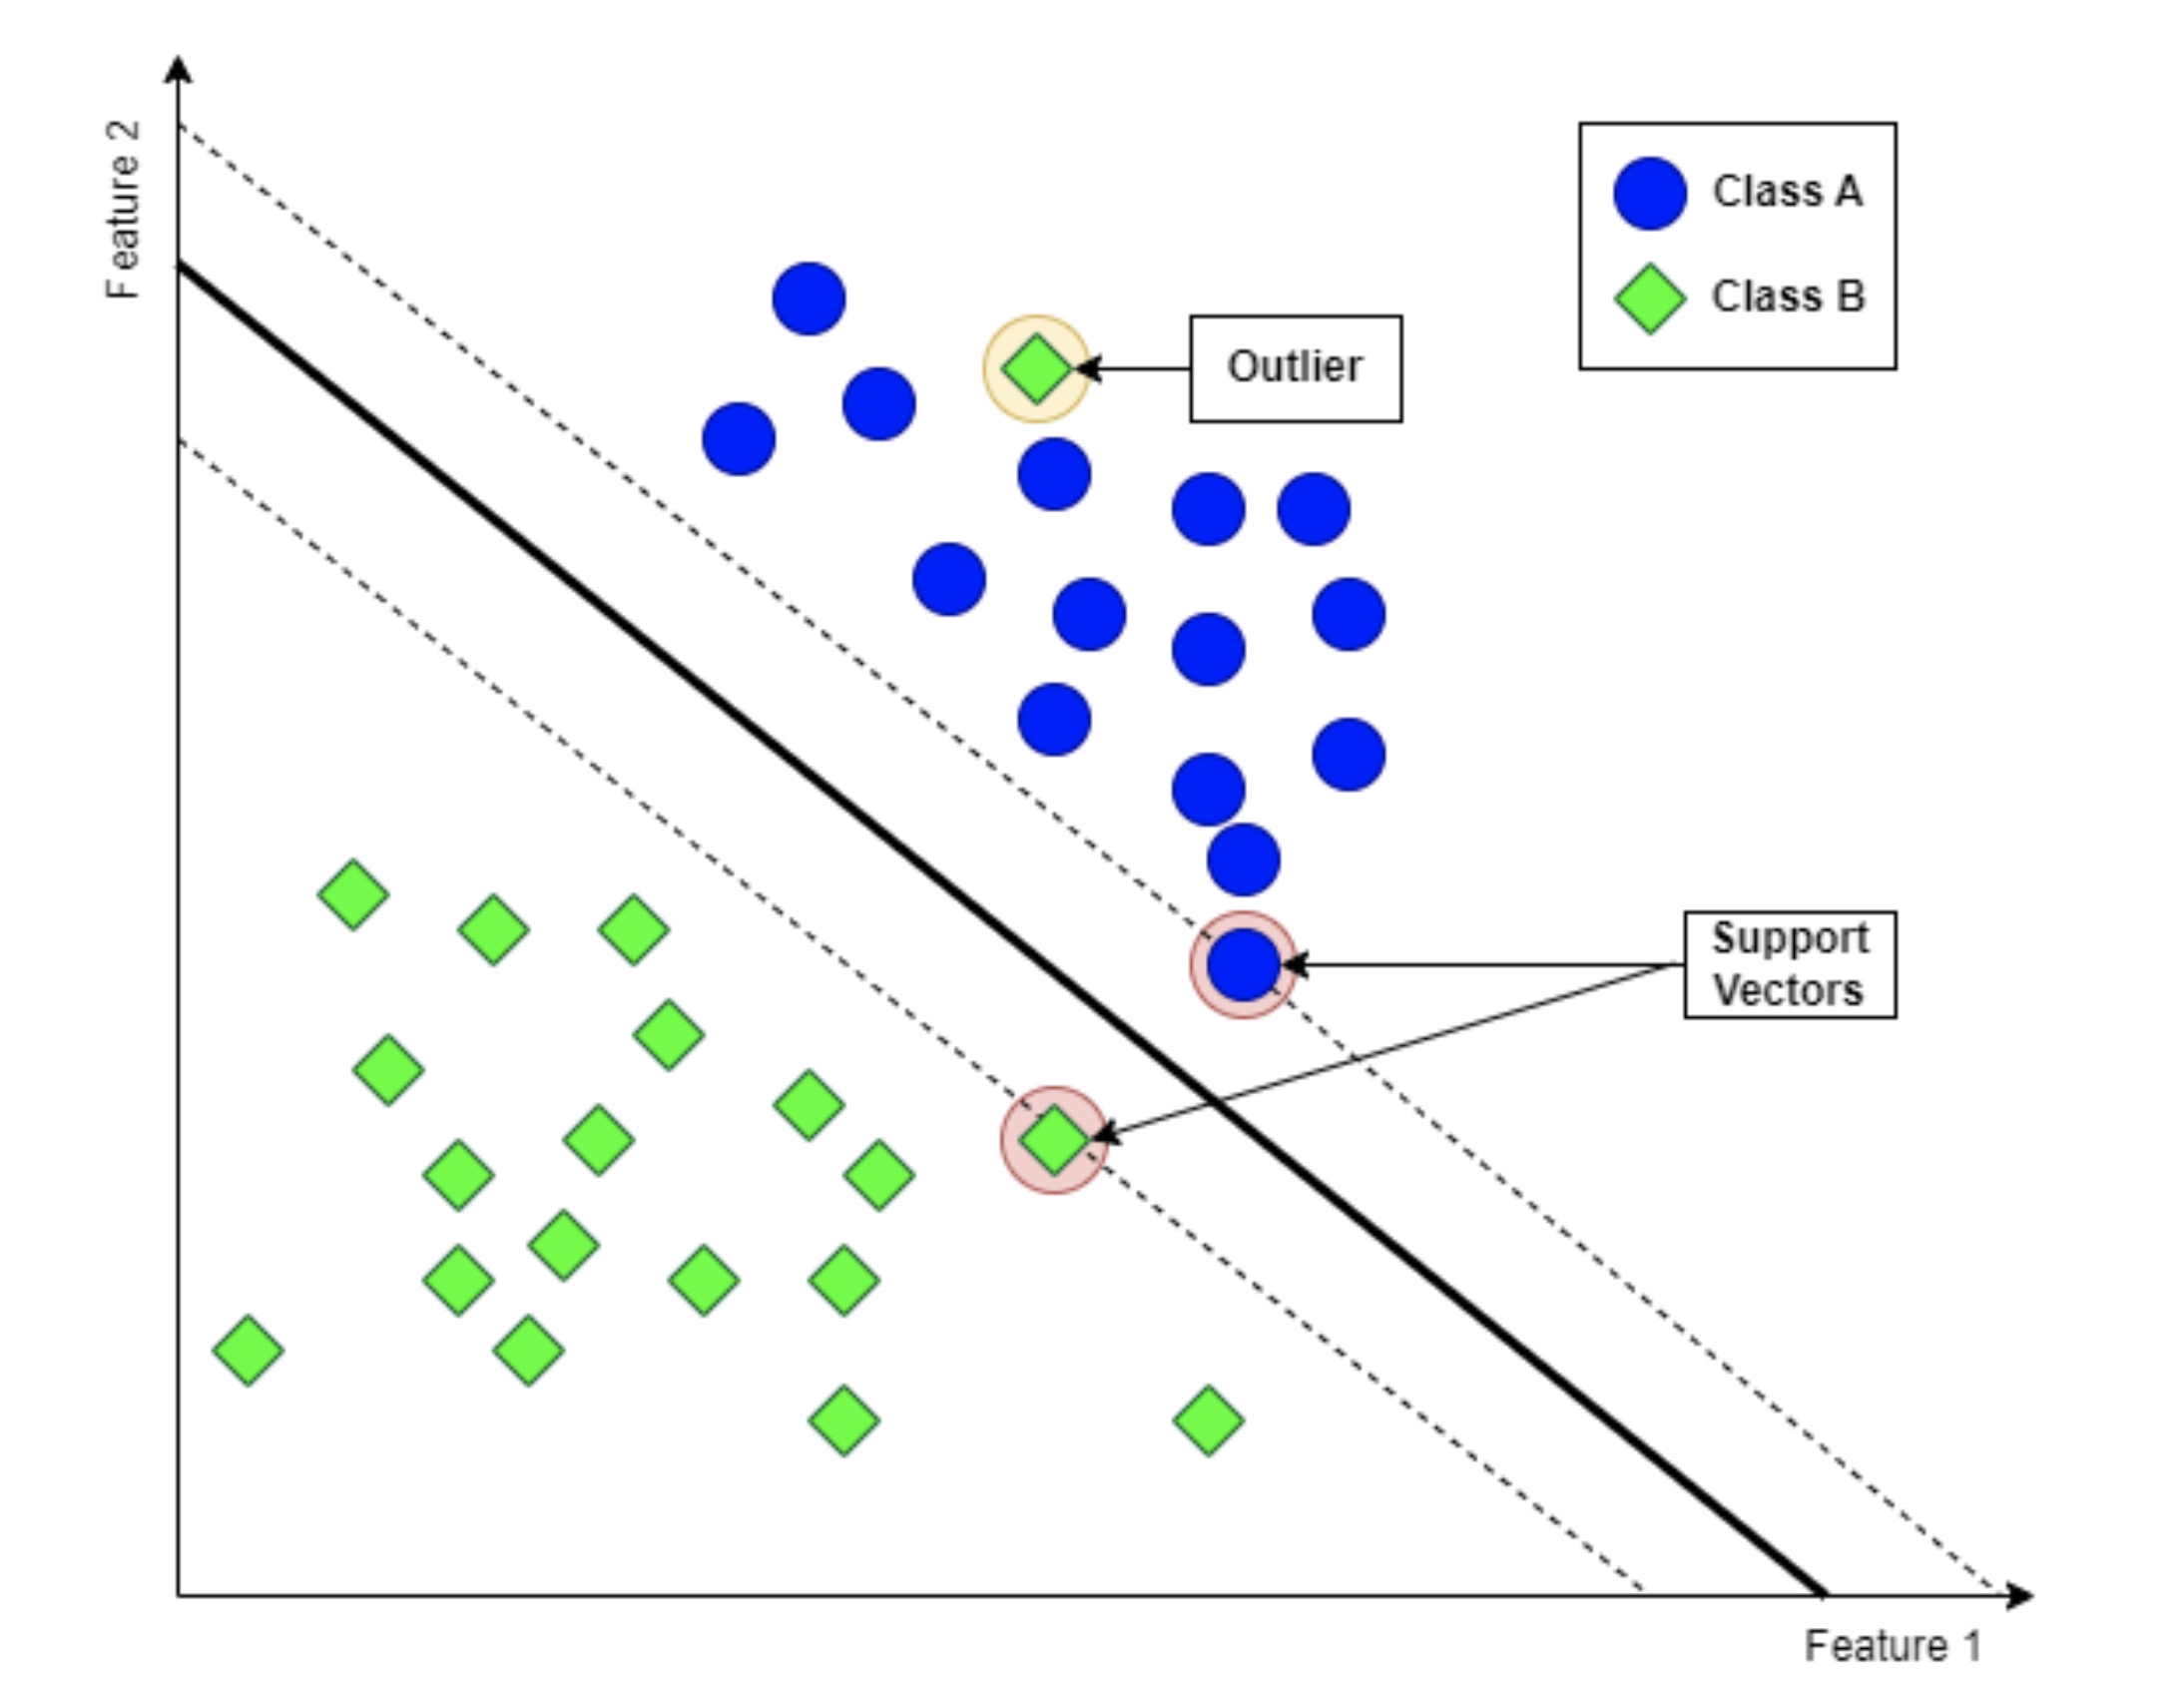
\includegraphics{fig/svm1.png}
\label{fig:sin}
\caption{Separable data.}
\end{marginfigure}

\begin{marginfigure}
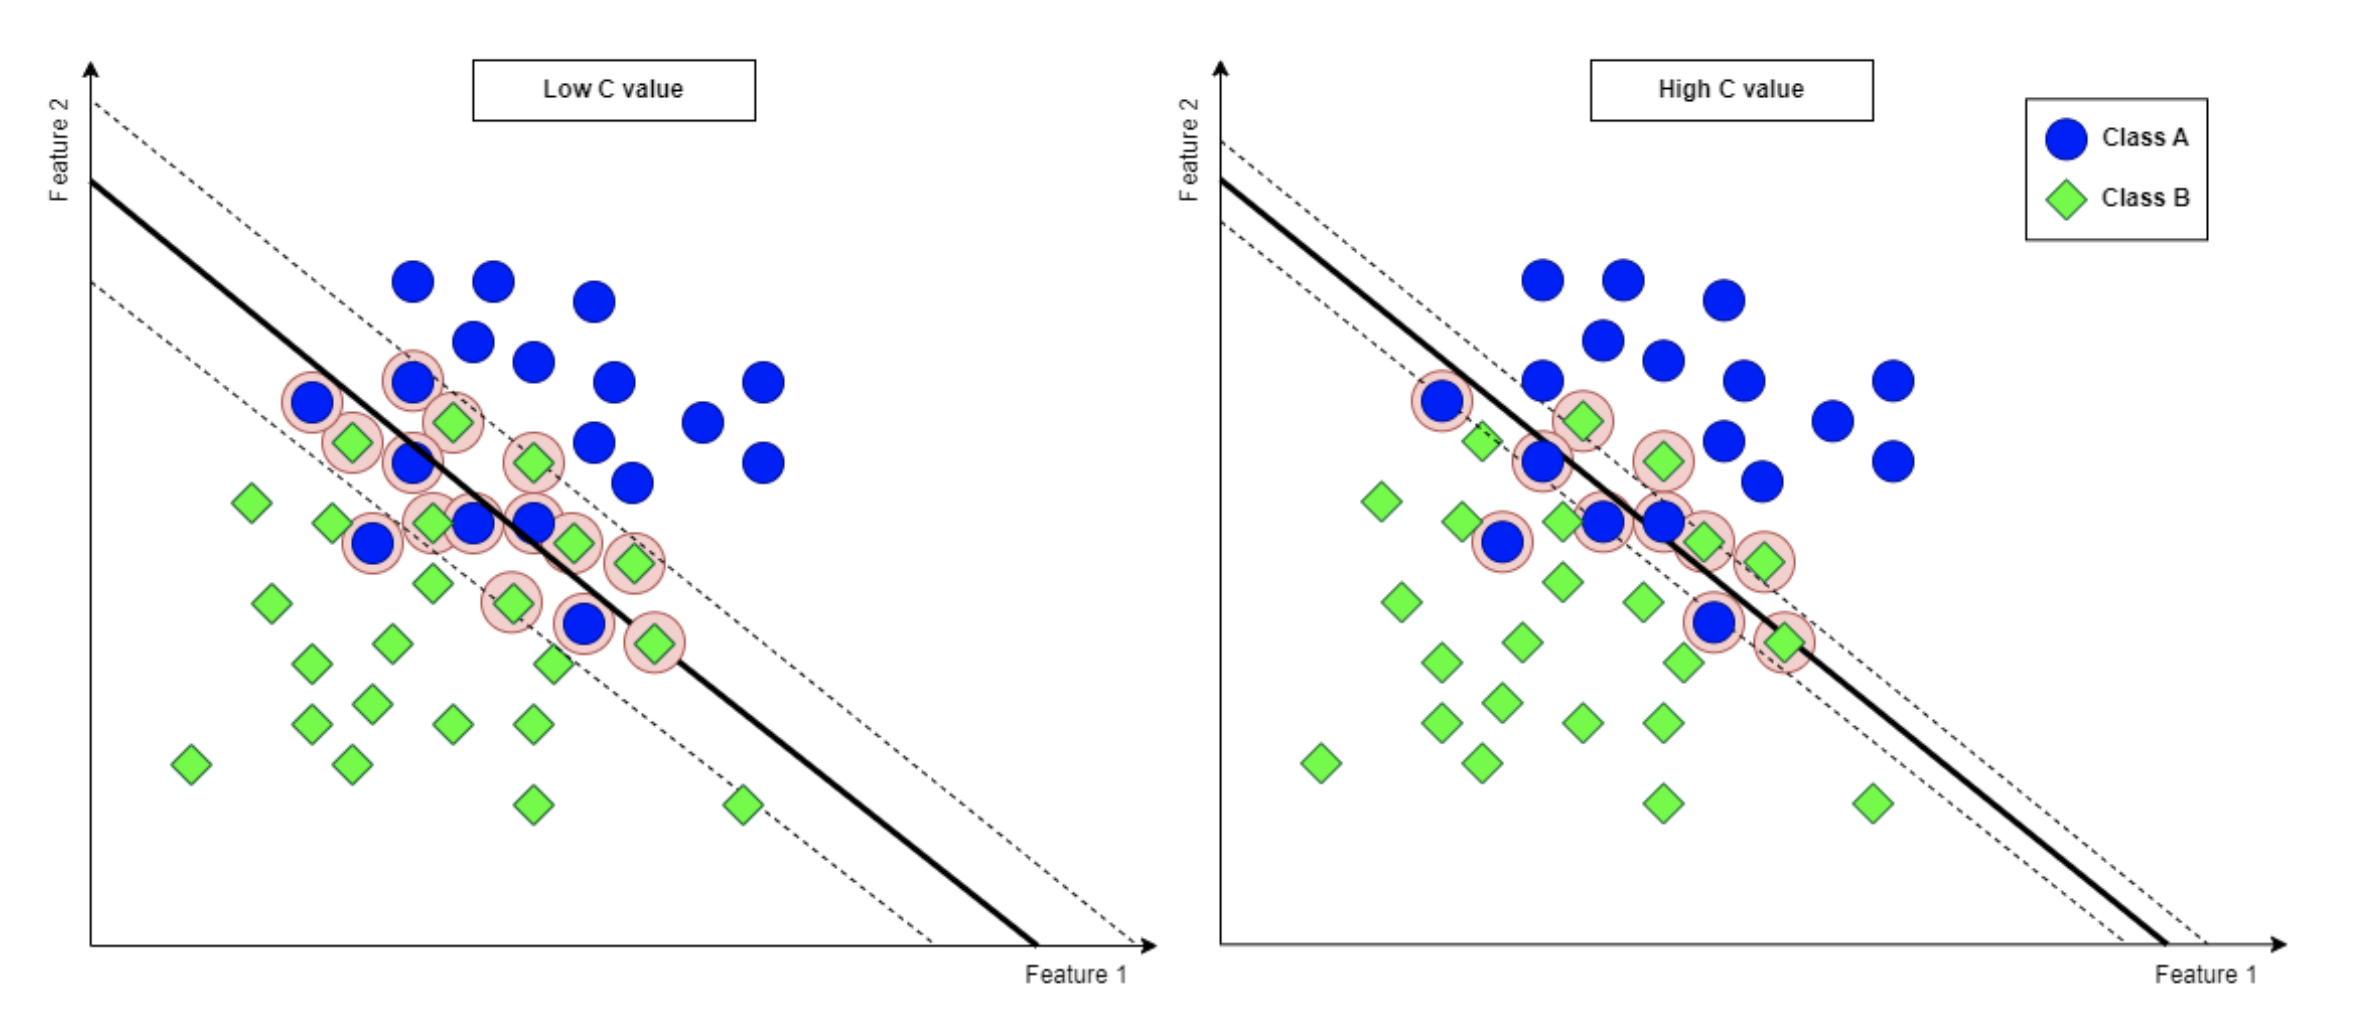
\includegraphics{fig/svm2.png}
\label{fig:sin}
\caption{Non-separable data.}
\end{marginfigure}

\subsection{Maximum Margin Principle}

Among all hyperplanes that separate the two classes, SVM seeks the one with the \textbf{maximum margin}. The margin is the distance between the hyperplane and the nearest data point from either class.

For a linearly separable dataset, we want:
\[
y_i(\langle w, x_i \rangle + b) \geq 1 \quad \text{for all } i = 1, \ldots, n
\]

The margin width is $\frac{2}{\|w\|}$. Therefore, maximizing the margin is equivalent to minimizing $\|w\|^2$.

\subsection{Optimization Problem (Hard Margin)}

The SVM optimization problem for linearly separable data is:
\begin{align}
\min_{w, b} \quad & \frac{1}{2}\|w\|^2 \\
\text{subject to} \quad & y_i(\langle w, x_i \rangle + b) \geq 1, \quad i = 1, \ldots, n
\end{align}

This is a convex quadratic programming problem.

\subsection{Support Vectors}

The \textbf{support vectors} are the training points that lie exactly on the margin boundaries, i.e., those for which:
\[
y_i(\langle w, x_i \rangle + b) = 1
\]

These are the critical points that define the optimal hyperplane. Removing any other points would not change the solution.

\section{Soft Margin SVM}

Real-world data is rarely perfectly separable. The \textbf{soft margin SVM} introduces slack variables $\xi_i \geq 0$ to allow some misclassifications:

\begin{align}
\min_{w, b, \xi} \quad & \frac{1}{2}\|w\|^2 + C \sum_{i=1}^{n} \xi_i \\
\text{subject to} \quad & y_i(\langle w, x_i \rangle + b) \geq 1 - \xi_i \\
& \xi_i \geq 0, \quad i = 1, \ldots, n
\end{align}

The parameter $C > 0$ controls the trade-off between:
\begin{itemize}
    \item Maximizing the margin (small $\|w\|$)
    \item Minimizing classification errors (small $\sum \xi_i$)
\end{itemize}

\begin{itemize}
    \item \textbf{Large C}: Smaller margin, fewer misclassifications (risk of overfitting)
    \item \textbf{Small C}: Larger margin, more misclassifications (more regularization)
\end{itemize}

\section{Kernel Trick for Non-Linear Classification}

When data is not linearly separable in the original space, SVMs use the \textbf{kernel trick} to implicitly map data to a higher-dimensional feature space where it becomes separable.

\subsection{Kernel Function}
A kernel function $k: \mathbb{R}^d \times \mathbb{R}^d \to \mathbb{R}$ computes the inner product in a transformed feature space:
\[
k(x, x') = \langle \phi(x), \phi(x') \rangle
\]
where $\phi: \mathbb{R}^d \to \mathcal{H}$ maps to a higher-dimensional (possibly infinite) feature space $\mathcal{H}$.


The decision function becomes:
\[
f(x) = \sum_{i=1}^{n} \alpha_i y_i k(x_i, x) + b
\]

where $\alpha_i$ are the Lagrange multipliers (non-zero only for support vectors).


\section{Connection to Hyperplane Separation Theorem}

SVMs are a direct application of the hyperplane separation theorem:

\begin{itemize}
    \item The two classes form convex hulls in the feature space
    \item The separation theorem guarantees a separating hyperplane exists (if classes don't overlap)
    \item SVM finds the \emph{optimal} such hyperplane by maximizing the margin
    \item This maximizes generalization to unseen data
\end{itemize}

\section{Key Properties}

\begin{itemize}
    \item \textbf{Convex optimization:} Guaranteed global optimum
    \item \textbf{Sparse solution:} Only support vectors matter
    \item \textbf{Kernel flexibility:} Handles non-linear boundaries
    \item \textbf{Regularization:} $C$ parameter controls overfitting
    \item \textbf{High-dimensional data:} Effective even when $d > n$
\end{itemize}

\section{Advantages and Limitations}

\textbf{Advantages:}
\begin{itemize}
    \item Effective in high-dimensional spaces
    \item Memory efficient (uses only support vectors)
    \item Versatile through different kernel functions
    \item Strong theoretical foundations
\end{itemize}

\textbf{Limitations:}
\begin{itemize}
    \item Computationally intensive for large datasets ($O(n^2)$ to $O(n^3)$)
    \item Sensitive to kernel and hyperparameter selection
    \item No probabilistic interpretation (without extensions)
    \item Primarily designed for binary classification
\end{itemize}

\section{Appendix}

\subsection{The XOR Problem}
Consider 2D input data with the XOR pattern:
\[
\mathbf{x} = \begin{bmatrix} x_1 \\ x_2 \end{bmatrix} \in \mathbb{R}^2
\]
This is not linearly separable in the original space.

\subsection{RBF Feature Map (Explicit Approximation)}
Using landmark points $\mathbf{c}_1, \mathbf{c}_2, \ldots, \mathbf{c}_m$, 
the RBF feature map is:
\[
\phi(\mathbf{x}) = \begin{bmatrix} 
\exp\left(-\gamma \|\mathbf{x} - \mathbf{c}_1\|^2\right) \\
\exp\left(-\gamma \|\mathbf{x} - \mathbf{c}_2\|^2\right) \\
\vdots \\
\exp\left(-\gamma \|\mathbf{x} - \mathbf{c}_m\|^2\right)
\end{bmatrix} \in \mathbb{R}^m
\]

where $\gamma > 0$ is the bandwidth parameter.

\subsection{RBF Kernel (Infinite Dimensional)}
The true RBF kernel corresponds to an \textbf{infinite-dimensional} feature space:
\[
K(\mathbf{x}, \mathbf{y}) = \exp\left(-\gamma \|\mathbf{x} - \mathbf{y}\|^2\right)
\]

Expanding the squared distance:
\begin{align}
K(\mathbf{x}, \mathbf{y}) &= \exp\left(-\gamma (\|\mathbf{x}\|^2 - 2\mathbf{x}^T\mathbf{y} + \|\mathbf{y}\|^2)\right) \\
&= \exp(-\gamma \|\mathbf{x}\|^2) \cdot \exp(2\gamma \mathbf{x}^T\mathbf{y}) \cdot \exp(-\gamma \|\mathbf{y}\|^2)
\end{align}

Using Taylor expansion of $\exp(2\gamma \mathbf{x}^T\mathbf{y})$:
\[
K(\mathbf{x}, \mathbf{y}) = \sum_{n=0}^{\infty} \frac{(2\gamma)^n}{n!} (\mathbf{x}^T\mathbf{y})^n 
\cdot \exp(-\gamma(\|\mathbf{x}\|^2 + \|\mathbf{y}\|^2))
\]

This represents an inner product in an \textbf{infinite-dimensional} Hilbert space!

\subsection{The Kernel Trick for RBF}
\begin{itemize}
    \item \textbf{Explicit feature map:} Would require infinite dimensions! Impossible to compute.
    \item \textbf{Kernel function:} $K(\mathbf{x}, \mathbf{y}) = \exp(-\gamma \|\mathbf{x} - \mathbf{y}\|^2)$ 
    \quad [Just one exponential!]
\end{itemize}

\textbf{Key insight:} The kernel trick allows us to work in infinite-dimensional 
feature spaces by only computing pairwise similarities!

\subsection{Properties of RBF Kernel}
\begin{enumerate}
    \item $K(\mathbf{x}, \mathbf{x}) = 1$ (self-similarity is always 1)
    \item $0 < K(\mathbf{x}, \mathbf{y}) \leq 1$ (similarity decreases with distance)
    \item As $\|\mathbf{x} - \mathbf{y}\| \to \infty$, $K(\mathbf{x}, \mathbf{y}) \to 0$
    \item $\gamma$ controls the "width" of the kernel:
    \begin{itemize}
        \item Large $\gamma$: narrow kernel, local influence
        \item Small $\gamma$: wide kernel, global influence
    \end{itemize}
\end{enumerate}


\section{Concentric Circles Example}

\subsection{Problem Setup}
Consider data distributed in two concentric circles in $\mathbb{R}^2$:
\begin{itemize}
    \item \textbf{Class 1 (Inner):} $\|x\| \approx r_1 = 1.0$
    \item \textbf{Class 2 (Outer):} $\|x\| \approx r_2 = 2.5$
\end{itemize}

Input: $\mathbf{x} = \begin{bmatrix} x_1 \\ x_2 \end{bmatrix} \in \mathbb{R}^2$

No linear classifier (straight line) can separate these circles!

\subsection{Radial Feature Map}
A simple yet effective feature map that exploits the radial structure:
\[
\phi(\mathbf{x}) = \begin{bmatrix} x_1 \\ x_2 \\ \|x\|^2 \end{bmatrix} 
= \begin{bmatrix} x_1 \\ x_2 \\ x_1^2 + x_2^2 \end{bmatrix} \in \mathbb{R}^3
\]

\textbf{Key insight:} The third coordinate captures the distance from origin!

\subsection{Linear Separability in Feature Space}
In the feature space $\mathbb{R}^3$, we can use a hyperplane:
\[
h(\phi(\mathbf{x})) = w_1 x_1 + w_2 x_2 + w_3(x_1^2 + x_2^2) + b = 0
\]

For concentric circles, we can choose $w_1 = w_2 = 0$ and $w_3 = 1$:
\[
h(\phi(\mathbf{x})) = x_1^2 + x_2^2 + b = \|x\|^2 + b
\]

Setting $b = -\left(\frac{r_1^2 + r_2^2}{2}\right)$, the decision boundary becomes:
\[
\|x\|^2 = \frac{r_1^2 + r_2^2}{2}
\]

This is a \textbf{circle} in the original space but a \textbf{hyperplane} 
in the feature space!

\subsection{Corresponding Kernel}
The inner product in feature space is:
\begin{align}
\langle \phi(\mathbf{x}), \phi(\mathbf{y}) \rangle &= 
\begin{bmatrix} x_1 \\ x_2 \\ x_1^2 + x_2^2 \end{bmatrix}^T
\begin{bmatrix} y_1 \\ y_2 \\ y_1^2 + y_2^2 \end{bmatrix} \\
&= x_1 y_1 + x_2 y_2 + (x_1^2 + x_2^2)(y_1^2 + y_2^2) \\
&= \mathbf{x} \cdot \mathbf{y} + \|\mathbf{x}\|^2 \|\mathbf{y}\|^2
\end{align}

\subsection{RBF Kernel for Concentric Circles}
The RBF kernel also works well:
\[
K(\mathbf{x}, \mathbf{y}) = \exp\left(-\gamma \|\mathbf{x} - \mathbf{y}\|^2\right)
\]

For concentric circles:
\begin{itemize}
    \item Points on the same circle have small $\|\mathbf{x} - \mathbf{y}\|$ 
    $\Rightarrow$ high similarity
    \item Points on different circles have large $\|\mathbf{x} - \mathbf{y}\|$ 
    $\Rightarrow$ low similarity
\end{itemize}

\subsection{Geometric Interpretation}
\begin{enumerate}
    \item \textbf{Original space:} Circular decision boundary (nonlinear)
    \item \textbf{Feature space:} Planar decision boundary (linear)
    \item \textbf{Transform:} Circles $\to$ separated regions along the $\|x\|^2$ axis
\end{enumerate}

The kernel trick allows us to work with circular boundaries while only 
computing linear separators in a higher-dimensional space!

\subsection{Why This Works}
The key property:
\[
r_1 < r < r_2 \iff r_1^2 < r^2 < r_2^2
\]

By adding $\|x\|^2$ as a feature, we effectively "lift" points based on 
their distance from the origin, making them linearly separable in 3D!




\end{document}


A basic neural network model can be described as a series of functional transformations. First, we construct $M_1$ linear combinations of the input variables $x_1,\dots,x_D$ in the form
\begin{equation}
a^0_j = \sum_{i=1}^D w_{ji}^{0}x_i + w_{j0}^{0}
\end{equation}
where $j=1,\dots, M_1$, and the superscript $(1)$ indicate that the corresponding parameters are in the \{firs layer \}of the network. We shall refer to the parameters $w_{ji}^{1}$ as the \textit{weights} and the parameters as the $w_{j0}^{1}$ biases. 

The quantities $a_j$ are known as \textit{activations}. Each of them is then transformed using a differentiable, nonlinear activation function $h(\cdot)$ to give
\begin{equation*}
z^0_j = h(a^0_j).
\end{equation*}
\begin{figure*}
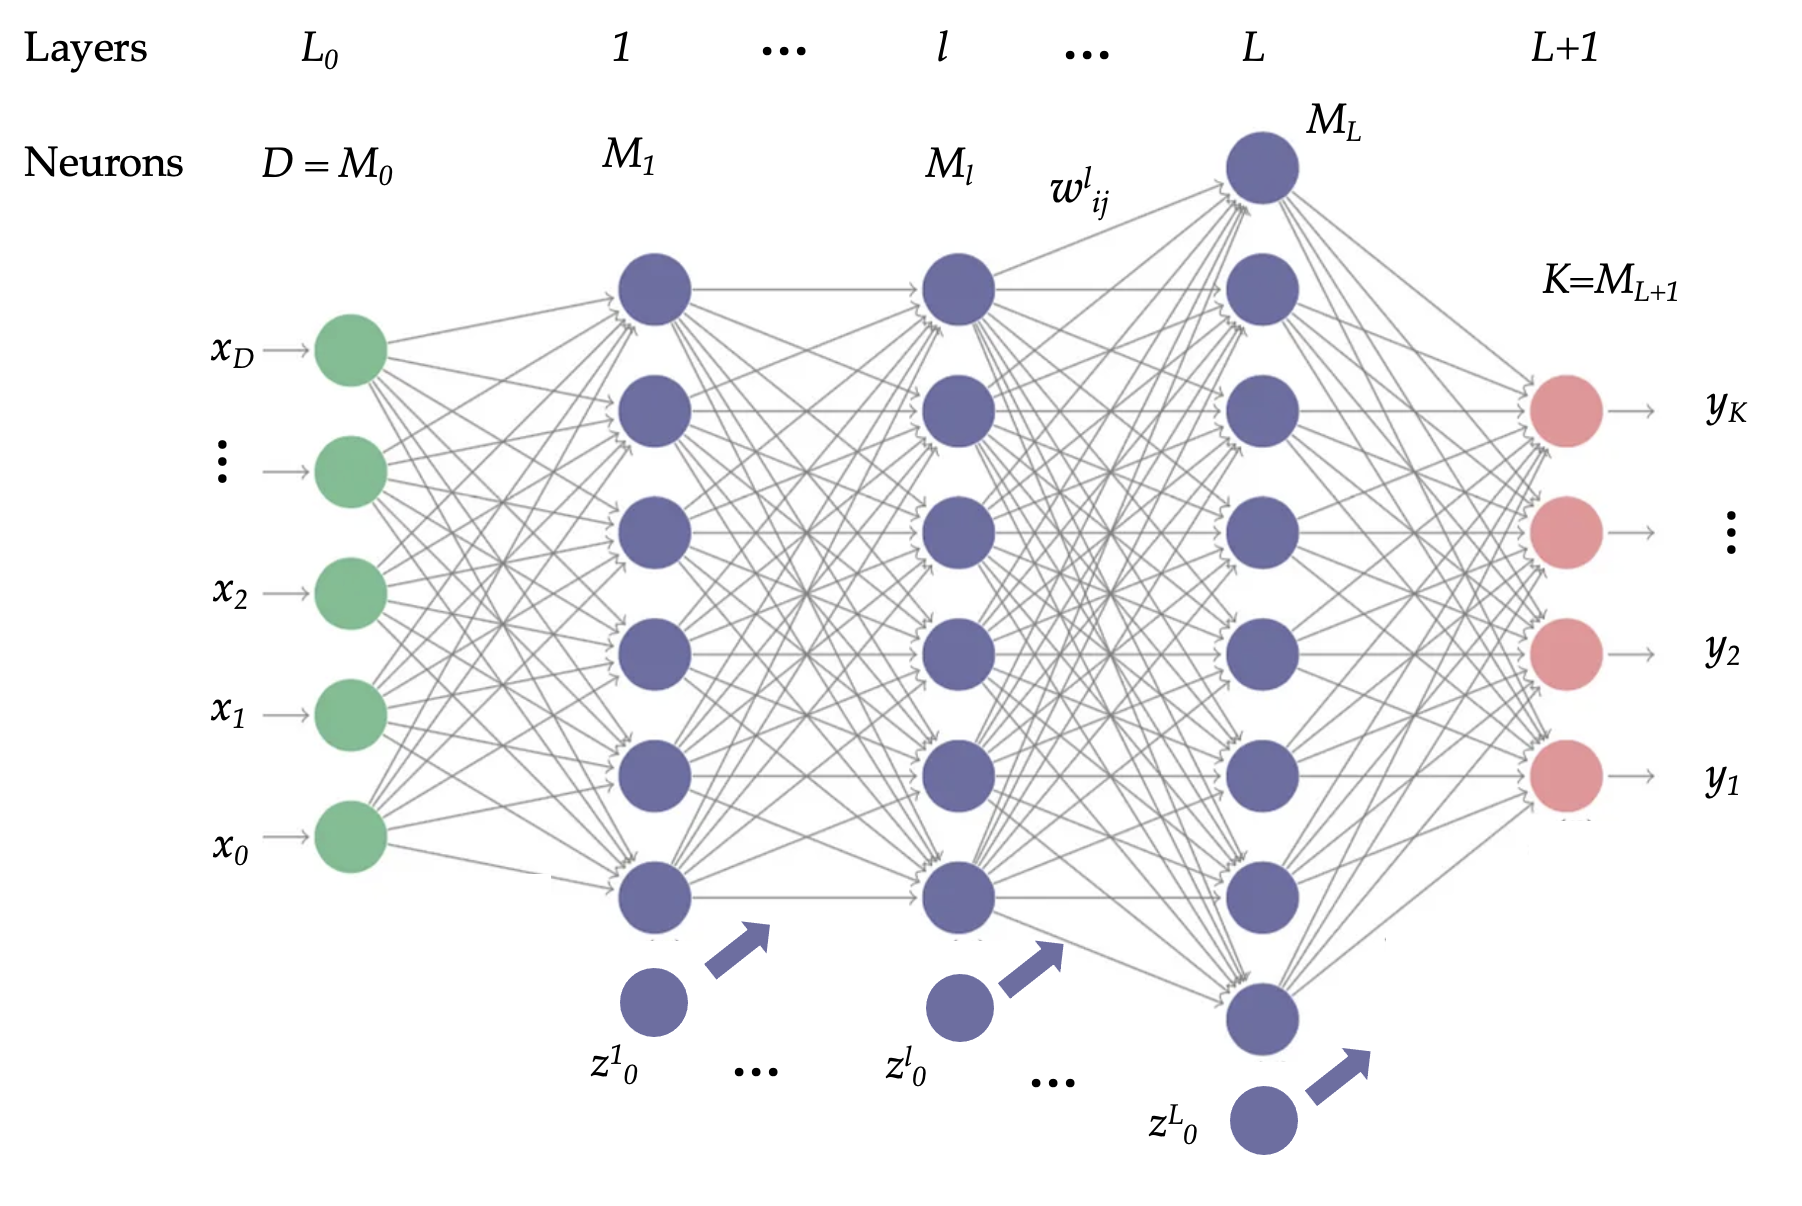
\includegraphics{fig/mlp2.png}
\label{fig:mlp}
\caption{Network diagram for the two-
layer neural MLP. The input,
hidden, and output variables
are represented by nodes, and $x_D$ the weight parameters are represented by links between the
nodes, in which links denote the bias input parameters
coming from additional input
and hidden variables $x_0$ and
$z_0$ . Arrows denote the direction of information flow through
the network during forward propagation.
}
\end{figure*}
These quantities correspond to the outputs of \textit{hidden units}. The nonlinear functions $h(\cdot)$ are generally chosen to be sigmoidal functions such as the logistic sigmoid or the ‘tanh’ function. These values are again linearly combined to give output unit activations
\begin{equation*}
a^1_k = \sum_{j=1}^M w_{kj}^{1}z^1_j + w_{k0}^{1}
\end{equation*}
where $k=1,\dots,K$, and $K$ is the total number of outputs. This transformation 
corresponds to the second layer of the network, and again the $w_{k0}^{(1)}$ are bias parameters.

Finally, the output unit activations are transformed using an appropriate activation function to give a set of network outputs $y_k.$ The choice of activation function is determined by the nature of the data and the assumed distribution of target variables. Thus for standard regression problems, the activation function is the identity so that $y_k = a_k$. Similarly, for multiple binary classification problems, each output unit activation is transformed using a logistic sigmoid function so that $y_k=\sigma(a_k)$.  Finally, for multiclass problems, a softmax activation function  is used.

We can combine these various stages to give the overall network function that, for sigmoidal output unit activation functions, takes the form
\begin{align*}
y_k(\mathbf x, \mathbf w) = h_2\left( \sum_{j=1}^M w_{kj}^{1} h_1\left(  \sum_{i=1}^D w_{ji}^{0}x_i + w_{j0}^{0} \right)  + w_{k0}^{1} \right),
\end{align*}
where the set of all weight and bias parameters have been grouped into a vector $\mathbf w$. Thus the neural network model is simply a nonlinear function from a set of input variables $\{x_i\}$ to a set of output variables $\{y_k\}$ controlled by a vector $\mathbf w$ of adjustable parameters.

The bias parameters in (1) can be absorbed into the set of weight parameters by defining an additional input variable $x_0$ whose value is clamped at $x_0 = 1$, so 
\begin{equation}
a_j = \sum_{i=0}^D w_{ji}^{1}x_i 
\end{equation}
We can absorb the second-layer biases into the second-layer weights so that the overall network becomes 
\begin{align*}
y_k(\mathbf x, \mathbf w) = h_2\left( \sum_{j=0}^M w_{kj}^{1} h_1\left(  \sum_{i=0}^D w_{ji}^{0}x_i \right) \right).
\end{align*}


As can be seen from Figure 1, the neural network model comprises two stages of processing, each of which resembles the perceptron model, and for this reason, the neural network is also known as the multilayer perceptron or MLP. A key difference compared to the perceptron, however, is that the neural network uses continuous sigmoidal nonlinearities in the hidden units, whereas the perceptron uses step-function nonlinearities. This means that the neural network function is differentiable concerning the network parameters, and this property will play a central role in network training.

The network architecture shown in Figure 1 is easily generalized, for instance by considering additional layers of processing each consisting of a weighted linear combination of the form (2) followed by an element-wise transformation using a nonlinear activation function.

As an example, consider a training set comprising a set of input vectors $\{\mathbf x_n\}$, where $n = 1,\dots,N$, together with a corresponding set of target vectors $\{\mathbf t_n\}$. We minimize the error function
\begin{align*}
E(\mathbf w) = \frac{1}{2}\sum_{n=1}^N \mid\mid \mathbf y(\mathbf x_n,\mathbf w)- \mathbf t_n\mid\mid^2,
\end{align*}
that is  we solve 
\begin{align*}
\hat{\mathbf w} = \arg\min_{\mathbf w} E(\mathbf w). 
\end{align*}
by setting $\nabla E(\mathbf w)=0$.
\begin{marginfigure}
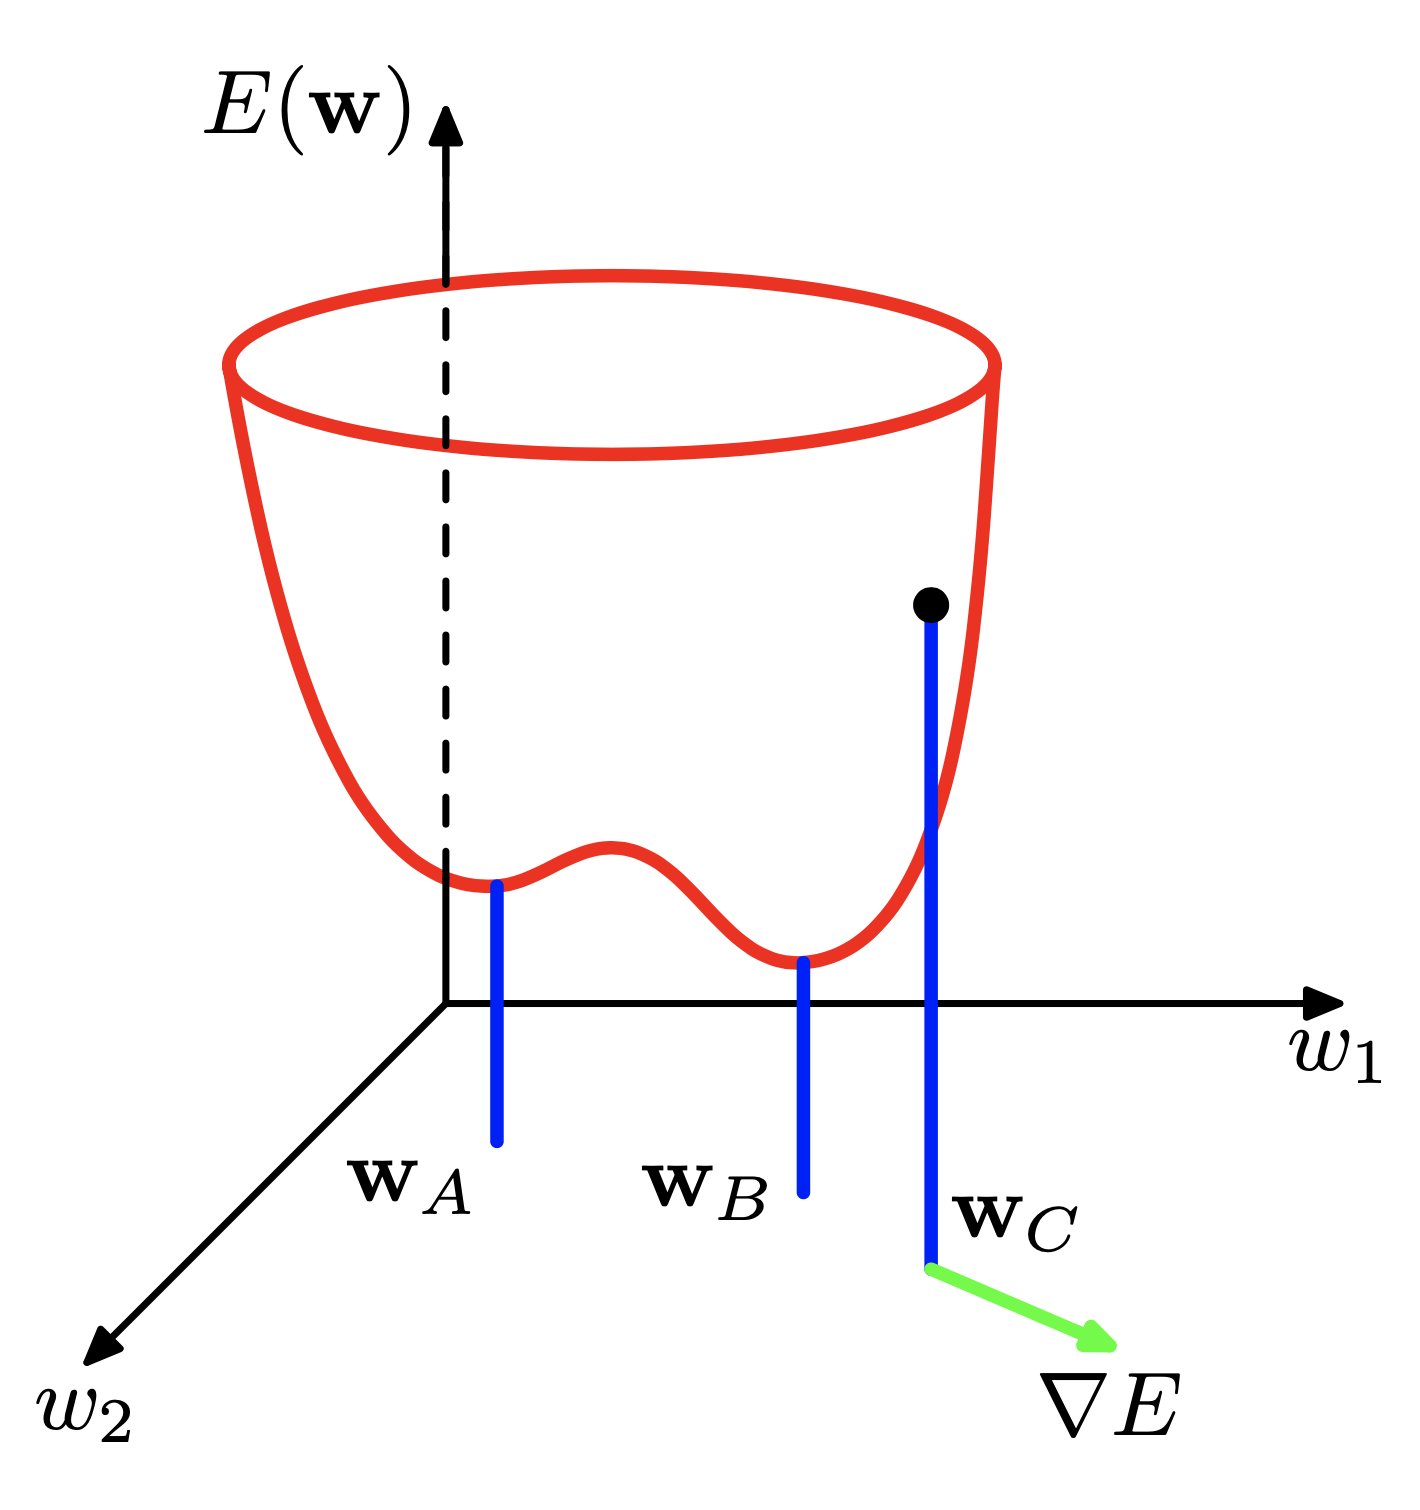
\includegraphics{fig/Ew.png}
\caption{Geometrical view of the error function $E(\mathbf w)$ as a surface sitting over weight space. Point $w_A$ is a local minimum and wB is the global minimum. At any point $w_C$, the local gradient of the error surface is given by the vector $\nabla E(\mathbf w)$,
}
\end{marginfigure}

In practice, the nonlinearity of the network function $ y(\mathbf x_n,\mathbf w)$ causes the error $E(\mathbf w)$ to be nonconvex, and so in practice, local maxima of the likelihood may be found, corresponding to local minima of the error function (Figure 2).


The simplest approach to using gradient information is to choose the weight update to comprise a small step in the direction of the negative gradient, so that
\begin{align*}
w^{(\tau+1)} = w^{(\tau)}-\eta \nabla E(w^{(\tau)})
\end{align*}
where the parameter $\eta > 0$ is known as the learning rate. After each such update, the gradient is re-evaluated for the new weight vector and the process is repeated. Note that the error function is defined concerning a training set, and so each step requires that the entire training set be processed to evaluate $\nabla E$. 

Techniques that use the whole data set at once are called batch methods. At each step the weight vector is moved in the direction of the greatest rate of decrease of the error function, and so this approach is known as gradient descent or steepest descent.

There is an online version of gradient descent that has proved useful in practice for training neural networks on large data sets. Error functions based on maximum likelihood for a set of independent observations comprise a sum of terms, one for each data point
\begin{align*}
w^{(\tau+1)} = w^{(\tau)}-\eta \nabla E_n(w^{(\tau)})
\end{align*}
Online gradient descent, also known as sequential \textit{gradient descent} or \textit{stochastic gradient descent}, makes an update to the weight vector based on one data point at a
time, so that

\begin{align*}
E(\mathbf w) = \sum_{n=1}^N E_n(\mathbf w).
\end{align*}
\section{Error Backpropagation}

\vspace{-0\baselineskip}\footnotetext{Source:Bishop. (2006). Pattern Recognition and Machine Learning, Springer.}
\vspace{0\baselineskip}

This update is repeated by cycling through the data either in sequence or by selecting points at random with replacements. There are of course intermediate scenarios in which the updates are based on batches of data points. A property of online gradient descent is the possibility of escaping from local minima since a stationary point for the error function for the whole data set will generally not be a stationary point for each data point individually.

Consider again a training set comprising a set of input vectors $\{\mathbf x_n\}$, where $n = 1,\dots,N$, together with a corresponding set of target vectors $\{\mathbf t_n\}$. We minimize the error function
\begin{align*}
E(\mathbf w) &= \frac{1}{2}\sum_{n=1}^N \mid\mid \mathbf y(\mathbf x_n,\mathbf w)- \mathbf t_n\mid\mid^2\\
&= \sum_{n=1}^N E_n(\mathbf w);
\end{align*}
that is,  we solve 
\begin{align*}
\hat{\mathbf w} = \arg\min_{\mathbf w} E(\mathbf w). 
\end{align*}
to find the neural network parameters by setting $\nabla E(\mathbf w)=0$.

Suppose that the network has $L$ fully connected layers,  with $M_l$ neurons each,  $l=2,\dots, L$. The input vector has dimension $D+1$ ($x_1 = 1$). We know that
\begin{align}
a_j^0 = \sum_{i=0}^{D} x_{i} w_{ji}^0,\,\,\, 
\end{align}
\begin{align}
z_j^0 = h(a_j^0),\,\, z_0^0=1
\end{align}
with $j=1,\dots,M_1$;
\begin{align}
a_j^l = \sum_{i=0}^{M_{l-1}} w_{ji}^lz_i^{l-1} ,\,\,\, j=1,\dots,M_l,
\end{align}
and 
\begin{align}
z_j^l = h(a_j^l) \equiv h^l(a_j^l ), \,\, z_0^l = 1.
\end{align}
with $l=1,2,\dots,L$. We find the gradient components as follows. We shall omit the subscript $n$ from the network variables to keep the notation uncluttered.
\begin{align}
\frac{\partial E_n}{\partial w_{ji}^l} &= \frac{\partial E_n}{\partial a_j^l}\frac{\partial a_j^l}{\partial w_{ji}^l}\nonumber\\
&=d_{j}^lz_i^{l-1}.
\end{align}
$j=1,\dots,M_l,$  $i=1,\dots,M_{l-1}$, $l=1,\dots, L$ and $z^l_0 = 1$. We define $d_{j}^l$ as
\begin{align*}
  \frac{\partial E_n}{\partial a_j^l} &=d_{j}^l.
\end{align*}
Notice that
\begin{align*}
  \frac{\partial a_j^0}{\partial w_{ji}^0} &= x_i.
\end{align*}
A total of $$\sum_{l=1}^{L+1} M_l \times M_{l-1}$$
coefficients need to be computed for a fully connected network. Also, notice that

\begin{align}
\frac{\partial E_n}{\partial z_j^{l}} &= \sum_{k=1}^{M_{l}} \frac{\partial E_n}{\partial  a_k^{l+1}} \frac{\partial a_k^{l+1}}{\partial z_j^{l}}\nonumber\\
&= \sum_{k=1}^{M_{l}} d_{k}^{l+1} \frac{\partial a_k^{l+1}}{\partial z_j^{l}}\nonumber\\
&= \sum_{k=1}^{M_{l}} d_{k}^{l+1} \frac{\partial}{\partial z_j^{l}} \left[ \sum_{i=1}^{M_{l}} z_i^{l}w_{ki}^{l+1} \right] \nonumber\\
&= \sum_{k=1}^{M_{l}} d_{k}^{l+1} w_{kj}^{l+1}.
\end{align}
$j=1,\dots,M_l,$ .Using matrix notation, we have that
\begin{align*}
\frac{\partial E_n}{\partial z_j^{l}} &=
\left[\frac{\partial a_1^{l+1}}{\partial z_j^l}, \dots, \frac{\partial a_1^{M_l+1}}{\partial z_j^l} \right]
\left[\frac{\partial E_n}{\partial a_1^{l+1}}, \dots, \frac{\partial a_1^{M_l+1}}{\partial a_1^{M_l+1}} \right]^T
&= \left(\frac{\partial \mathbf a^{l+1}}{\partial \mathbf z^{l+1}}\right) (\nabla_{\mathbf a^{l+1}} \mathbf E_n)^T.
\end{align*}
We can derive the following recursive equation.
\vspace{0\baselineskip}
\begin{align}
d_j^l &= \frac{\partial E_n}{\partial a^l_j} \\
&= \frac{\partial E_n}{\partial z^l_j}\frac{\partial z_j^l}{\partial a_j^l}\nonumber\\
&= \frac{\partial E_n}{\partial z^l_j}h'(a_j^l)\nonumber\\
&= h'(a_j^l) \sum_{k=1}^{M_{l}} d_{k}^{l+1} w_{kj}^{l+1}.
\end{align}
Notice that the error function  for each $n$  equals
\begin{align*}
E_n(\mathbf w) = \frac{1}{2}\sum_{k=1}^{M_L}(y_{k}-t_{k})^2.
\end{align*}
Therefore 
\begin{align*}
\frac{\partial }{\partial w_{ji}^L}E_n(\mathbf w)= (y_{j}-t_{j})z_i^L = d^L_jz_i^{L-1}.
 \end{align*}
To avoid a cluttered notation, we omit the subscript $n$ from the network variables.



\subsection{Error Backpropagation}

\begin{mybox}{Backpropagation }{theoexample}
\begin{enumerate}
\item  Apply an input vector $x_n$ to the network and forward propagate through the network using (3-6) to find the activations of all the hidden and output units.
\item Evaluate the $d$'s for all the output units: $d_{j}^L = y_{j} - t_{j}$. 
\item Backpropagate the $d$'s using (9) to obtain the $d$'sfor each hidden unit in the
network.
\begin{align*}
d_j^l  &\leftarrow h'(a_j^l) \sum_{k=1}^{M_{l}} d_{k}^{l+1} w_{kj}^{l+1}.
\end{align*}

\begin{align*}
d_j^l  &\leftarrow h'(a_j^l) \sum_{\forall k \rightarrow j} d_{k}^{l+1} w_{kj}^{l+1}.
\end{align*}
$j=1,\dots,M_l,$  $l=2,\dots, L$.


\item  Use (7) to evaluate the required derivatives.
\begin{align*}
\frac{\partial E_n}{\partial w_{ji}^l}
&=d_{j}^lz_i^{l-1}.
\end{align*}
\end{enumerate}
\end{mybox}








%\\&= \;\;  \left[ \sigma'(a_1^1)(d_1^2w^2_{11}+d_2^2w^2_{21}+ d_3^2w^2_{31})\;\; \sigma'(a_2^1)(d_1^2w^2_{12}+d_2^2w^2_{22}+ d_3^2w^2_{31}) \;\;\;\sigma'(a_3^1)(d_1^2w^2_{13}+d_2^2w^2_{23}+ d_3^2w^2_{31}) \;\;\;\sigma'(a_4^1)(d_1^2w^2_{13}+d_2^2w^2_{23}+ d_3^2w^2_{31}) \right]
%\begin{align*}
%\mathbf d^0  &= \left[ d_1^0\; d_2^0\; d_3^0 \right]
%\\&=  \left[ d_1^1\; d_2^1\; d_3^1 \; d_4^1 \right]
%\begin{bmatrix}
%w^1_{11} & w^1_{12} & w^1_{13}  \\
%w^1_{21}  & w^1_{22} & w^1_{23} \\
%w^1_{31} & w^1_{32} & w^1_{33} \\
%w^1_{41} & w^1_{42} & w^1_{43} \\ 
%\end{bmatrix} 
%\begin{bmatrix}
%\sigma'(a_1^0) & 0 & 0 \\
%0  & \sigma'(a_2^0) & 0  \\
%0  & 0 & \sigma'(a_3^0)  \\
%\end{bmatrix} 
%\end{align*}


%\begin{align*}
%\mathbf G^0 &= \left[ d_1^0\; d_2^0\; d_3^0  \right]^T \left[ \sigma(a_1^0) \,\, \sigma(a_2^0) \,\, \sigma(a_3^0) \right]\\
 %\end{align*}

The gradient descent  update equation is 
\begin{align*}
\mathbf W^{l} &\Leftarrow \mathbf W^{l} - \alpha \mathbf G^l,\,\,\, l=0,1,2.
 \end{align*}
where $\alpha $ is the learning rate.

\subsection{Regularization in Neural Networks }

The number of input and output units in a neural network (Figure 1) is generally determined by the dimensionality of the data set. In contrast, the number $M$ of hidden units is a free parameter that can be adjusted to give the best predictive performance. Note that $M$ controls the number of parameters (weights and biases) in the network, and so we might expect that in a maximum likelihood setting, there will be an optimum value of M that gives the best generalization performance, corresponding to the optimum balance between under-fitting and over-fitting.

There are, however, other ways to control the complexity of a neural network model to avoid over-fitting.
The simplest regularizer is the quadratic, giving a regularized error of the form
\begin{align*}
E\lambda( \mathbf w) &= E(\mathbf w) + \frac{\lambda}{2} \mathbf w^T \mathbf w= E(\mathbf w) + \frac{\lambda}{2} 
\mid\mid \mathbf w\mid\mid^2\\
&= \sum_{n=1}^N E_n(\mathbf w) + \frac{\lambda}{2} 
\mid\mid \mathbf w\mid\mid^2
\end{align*}

Notice that:
\begin{align*}
\frac{\partial E_n^\lambda}{\partial w_{ji}^l} &= \delta_{j}^lz_i^{l-1} + \frac{\partial}{\partial w_{ji}^l} \mid\mid \mathbf w\mid\mid^2.\\
&= \delta_{j}^lz_i^{l-1} + 2 w_{ji}^l
\end{align*}
with
\begin{align*}
\delta^j_l&= h'(a_j^l) \sum_{k=1}^{M_{l+1}} \delta_{k}^{l+1} w_{kj}^{l+1}.
\end{align*}

This particular choice of regularizer is known in the machine learning literature as weight decay because, in sequential learning algorithms, it encourages weight values to decay toward zero unless supported by the data. In statistics, it provides an example of a parameter shrinkage method because it shrinks parameter values. It has the advantage that the error function remains a quadratic function of $\mathbf w$. 




\end{document}
\end{document}






